\chapter{Resultados}

	El presente capítulo expone los resultados obtenidos tras el desarrollo del sistema de desalinización propuesto. Los resultados se organizan para proporcionar una visión integral del diseño y funcionamiento del sistema. Para lograr este cometido, se presenta de manera coherente de acuerdo al proceso seguido para obtener estos resultados.
	
	En primer lugar, se muestra la vista general del funcionamiento del sistema para comprender la interacción entre los componentes del desalinizador. A continuación, se entra en detalle con el diseño propuesto y se validan los componentes a través de simulaciones de transferencia de calor que sustentarán al modelo de control difuso que regula la alimentación del sistema.

	
	\section{Comportamiento e interacciones del desalinizador propuesto}
	
		Como se ha mencionado anteriormente, esta propuesta está encaminada a sortear los problemas identificados en la destilación solar. Para ello, se separa la evaporación del agua del calentamiento. En la~\cref{fig:VistaGeneral} se observa que la interacción entre el recibidor solar y el mecanismos de evaporación es independiente.
	
		\begin{figure}
			\centering
			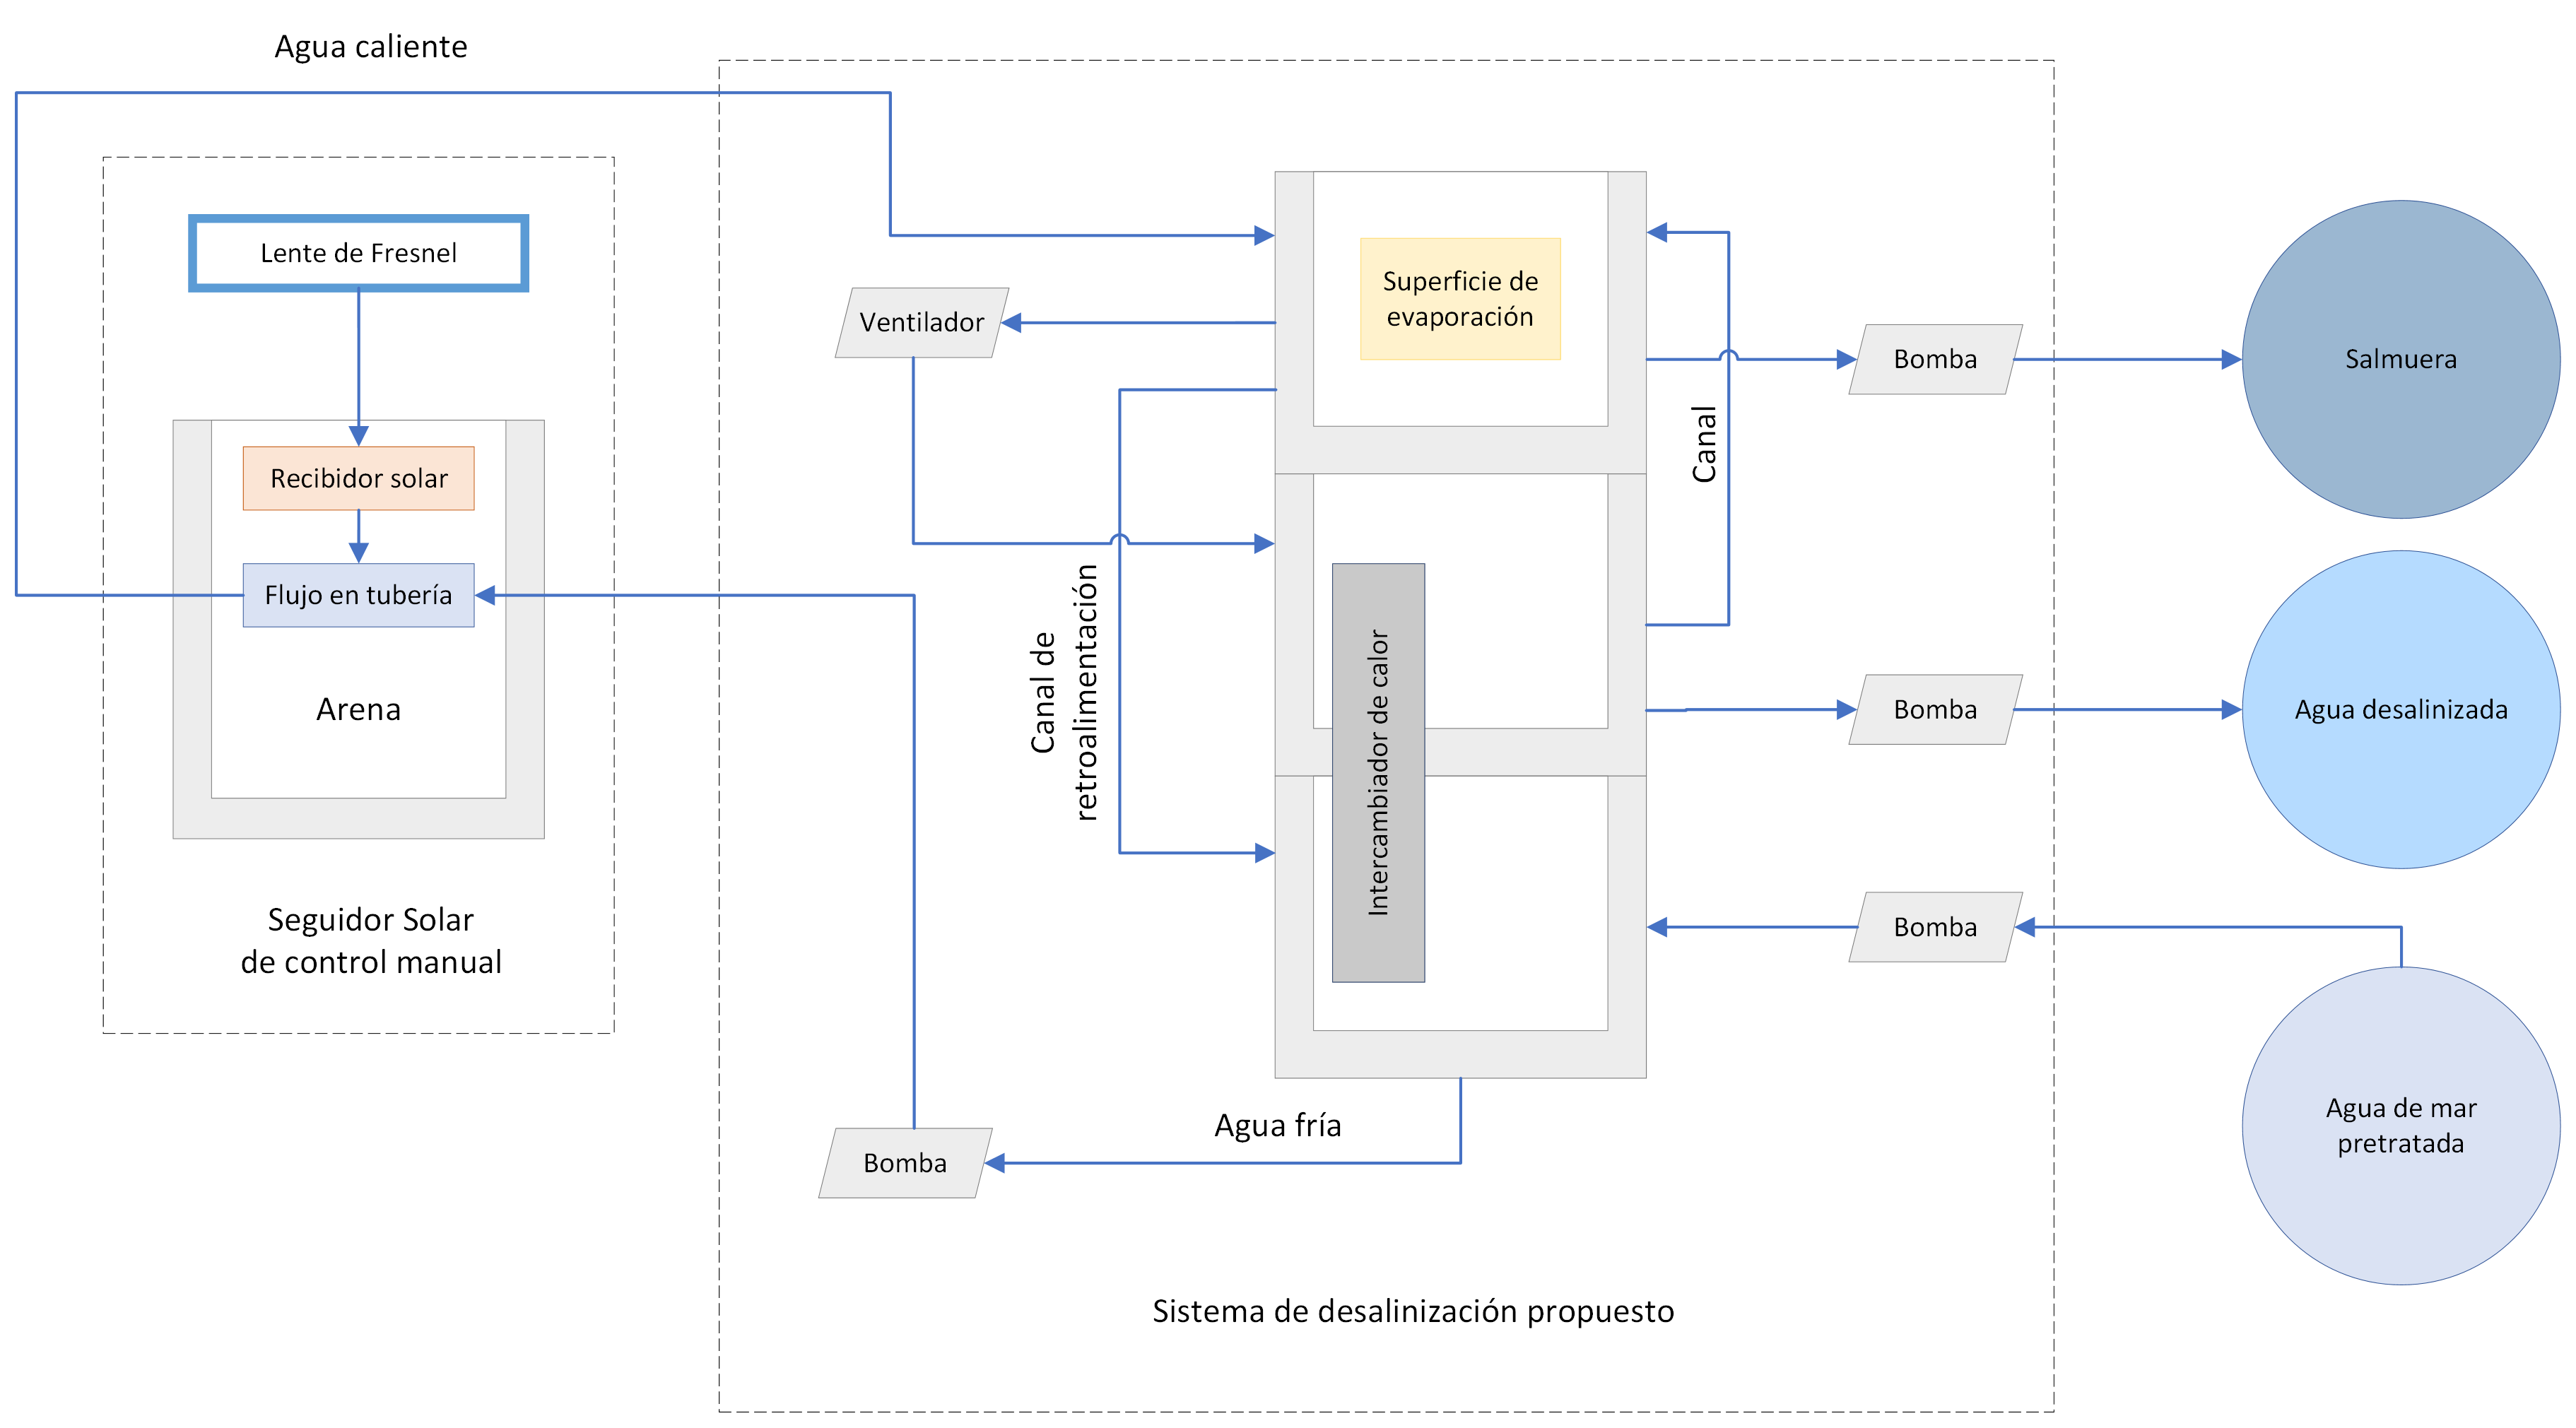
\includegraphics[
				width=\linewidth,
				height=12cm,
				keepaspectratio
			]{Resultados/Sistema/VistaGeneral.png}
			\caption{Vista general del proceso de desalinización}
			\label{fig:VistaGeneral}
		\end{figure}
		
		Gracias a este esquema se logra evitar la interferencia del vapor de agua a la superficie de calentamiento. Para validar este modelo, se usó Autodesk Inventor para la parte del diseño del sistema y Autodesk CFD para el modelado de la transferencia de calor y el flujo de aire.
		
		\subsection{Principio de funcionamiento}
			
			El desalinizador se diseñó buscando aprovechar en la medida de lo posible el calor generado por el concentrador solar, a su vez, se buscó promover la evaporación evitando volumenes grandes de agua.
			
			El desalinizador inicia su operación con un volumen de agua salada a temperatura ambiente, mediante una bomba con la capacidad de regular su caudal, una vez se alcanzan ciertas condiciones, se bombea agua hacia una tubería que se calienta mediante el recibidor solar. Una vez caliente el agua se dirige hacia una cámara donde se evapora el agua. Para favorecer este fenómeno se mantiene un volumen de agua bajo mientras que un ventilador redirige el vapor generado a una segunda cámara. El flujo de aire creado por el ventilador permite desalojar el aire saturado y renovarlo con aire más seco.
			
			El agua caliente excedente se vuelve a inyectar al inicio del ciclo mientras que el vapor generado es condensado mediante un intercambiador de calor que a su vez transmite ese calor al agua entrante.
		
	
		\subsection{Componentes y módulos del desalinizador}
			
			Tras varias propuestas se llegó a un diseño modular vertical. En la~\cref{fig:WaterModule} se puede observar el primer módulo llamado ``Módulo de reaprovechamiento térmico y bombeo'' el cual se diseñó para aprovechar el calor del vapor generado tras pasar por el ``Módulo de concentración solar'' (\cref{fig:SolarModule}) el cual se integra a un seguidor solar para calentar el agua indirectamente por medio de la lente de Fresnel.
		
		
			\begin{figure}[H]
				\centering
				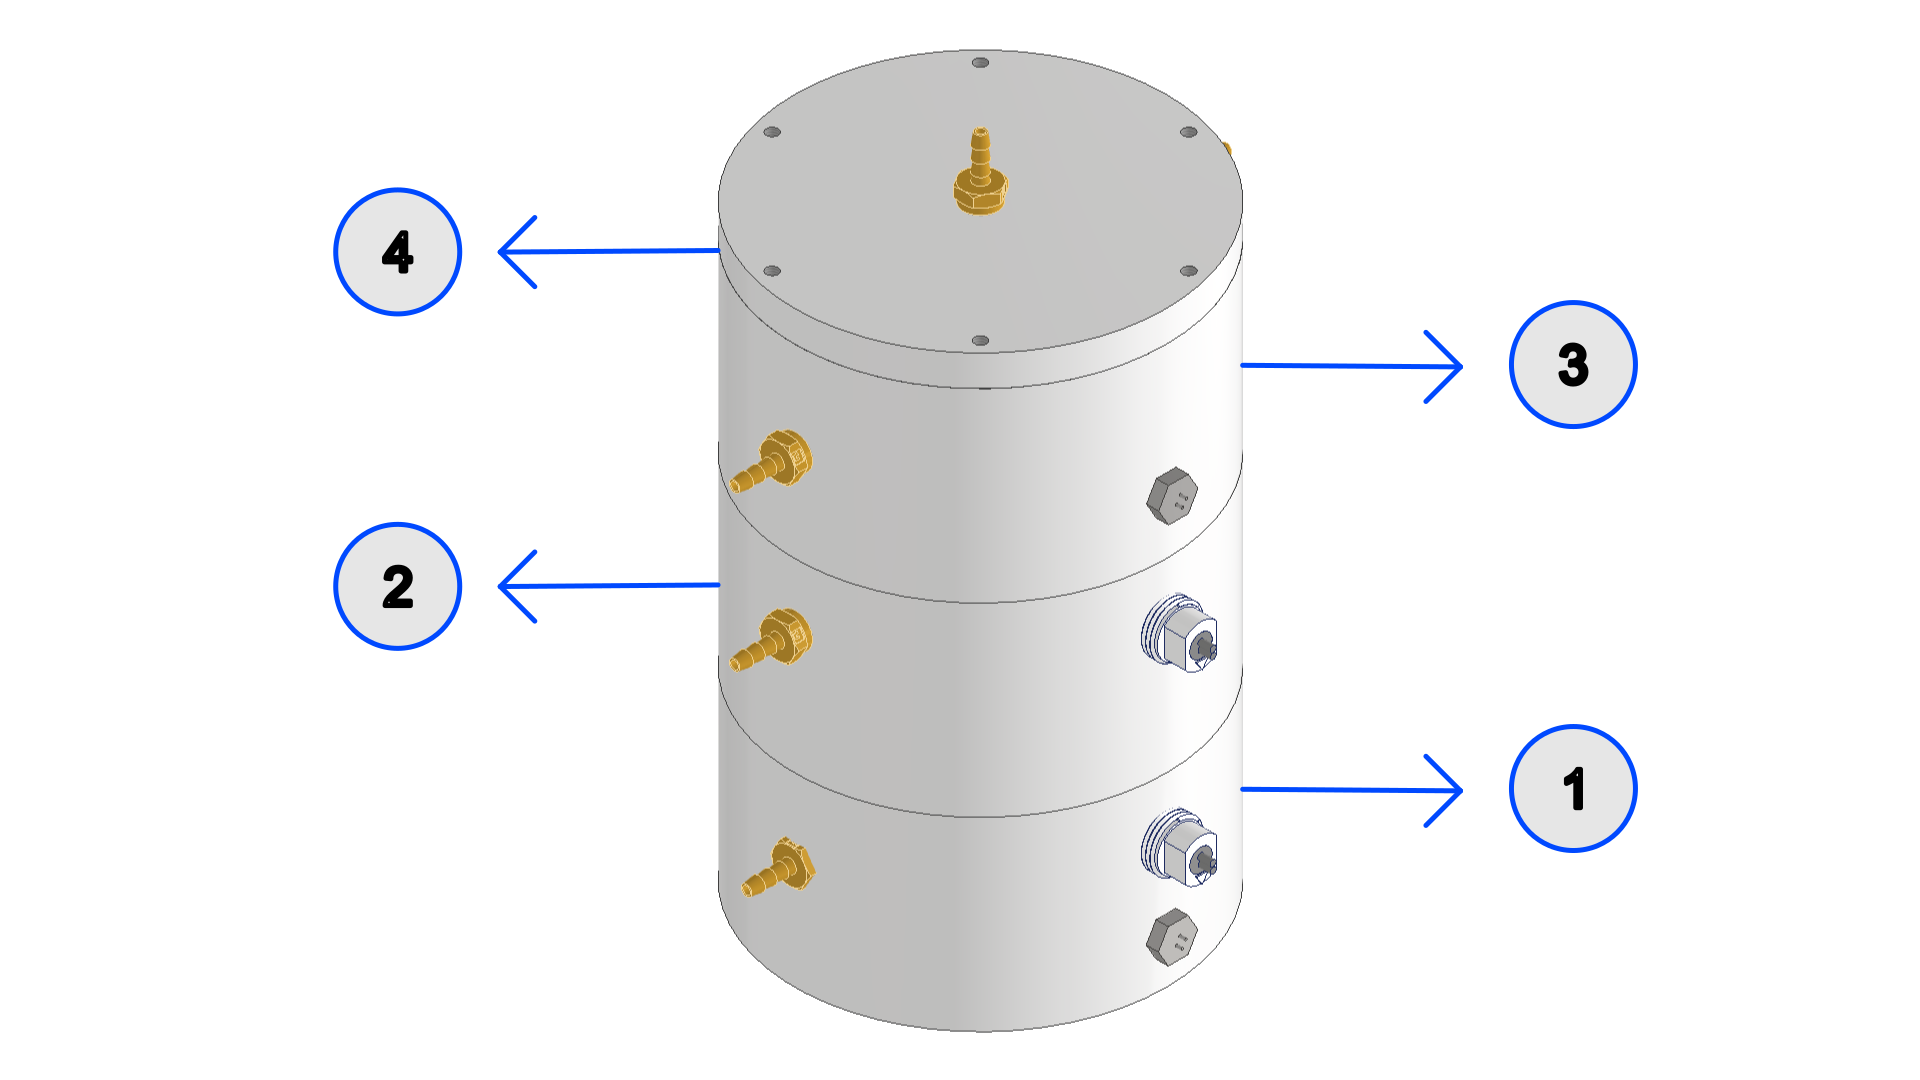
\includegraphics[
					width=\linewidth,
					height=70mm,
					keepaspectratio
				]{Resultados/Sistema/WaterModule.png}
				\caption{Propuesta del sistema desalinizador. Módulo de reaprovechamiento térmico y bombeo.}
				\label{fig:WaterModule}
			\end{figure}
			
			\begin{enumerate}[columns=2]
				\item Contenedor de agua de mar
				\item Contenedor de agua destilada
				\item Cámara de evaporación
				\item Tapa
			\end{enumerate}
			
			\begin{figure}[H]
				\centering
				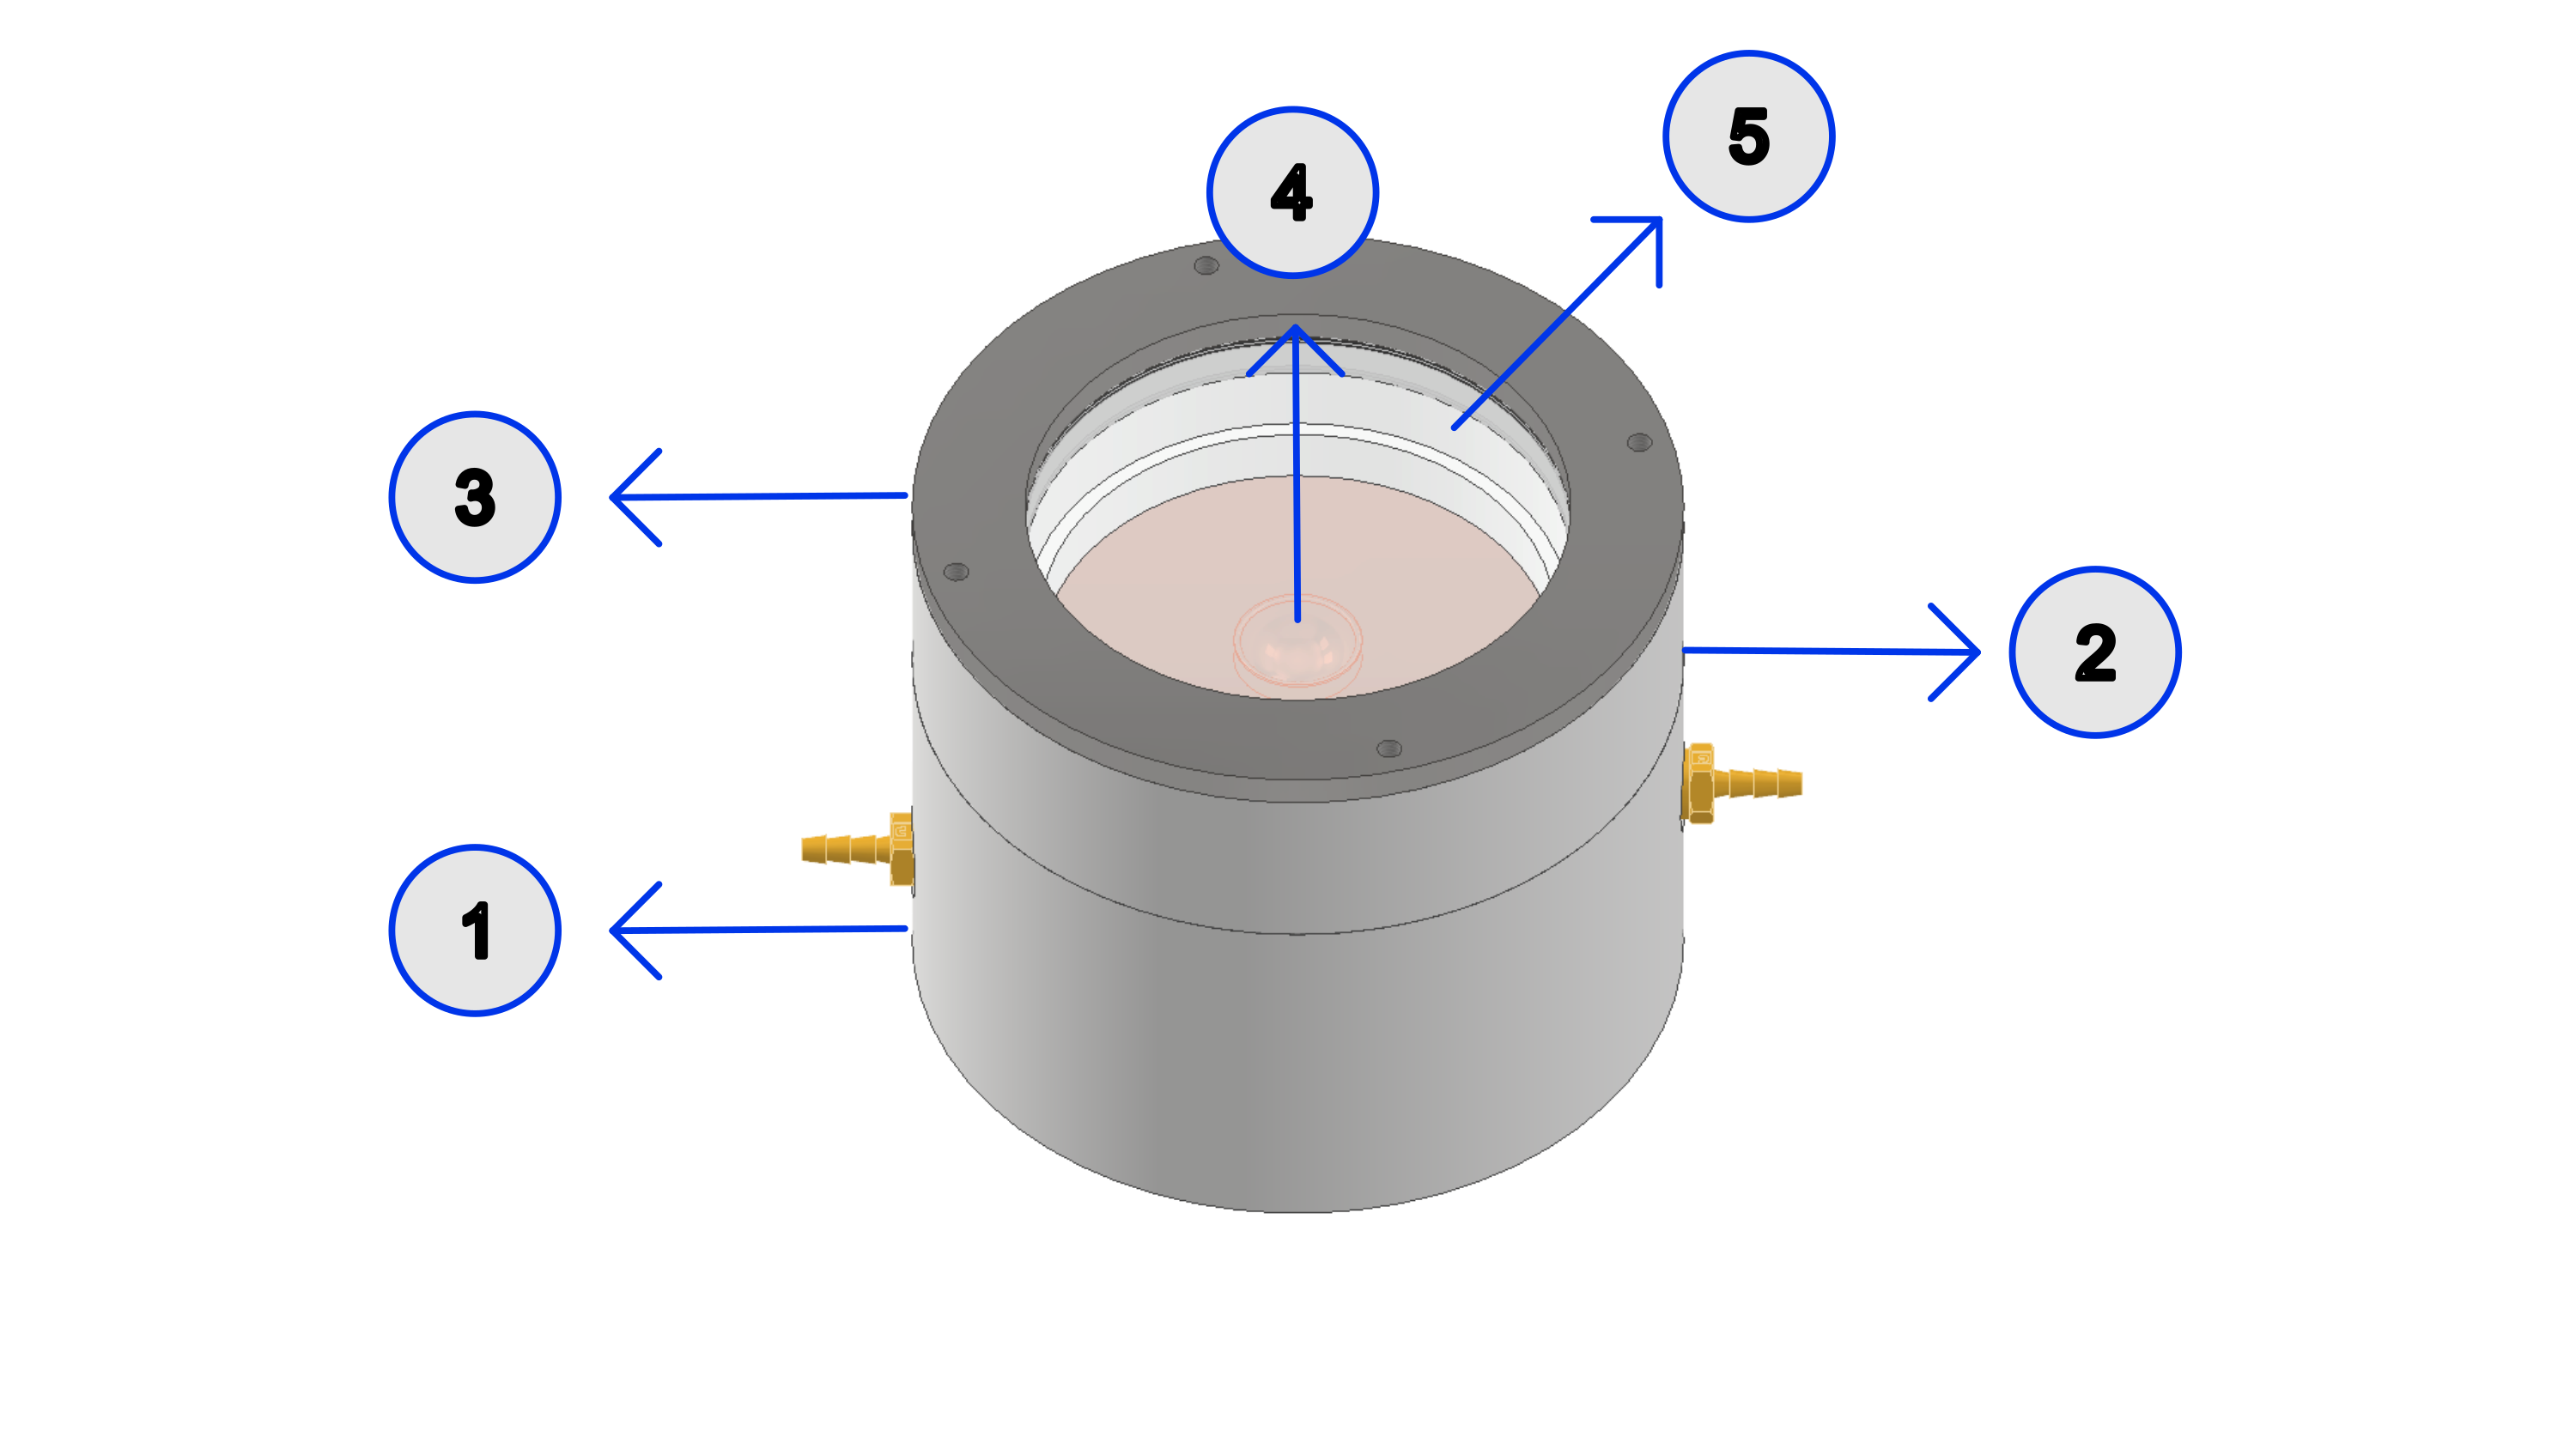
\includegraphics[
					width=\linewidth,
					height=70mm,
					keepaspectratio
				]{Resultados/Sistema/SolarModule.png}
				\caption{Propuesta del sistema desalinizador. Módulo de concentración solar.}
				\label{fig:SolarModule}
			\end{figure}
			
			\begin{enumerate}[columns=2]
				\item Cámara de transferencia de calor
				\item Soporte de lente
				\item Tapa
				\item Recibidor solar
				\item Cristal de borosilicato
			\end{enumerate}
			
			En los siguientes apartados se detallan los elementos que componen a este sistema y las funciones que desempeñan.
	
			\subsubsection{Contenedor de agua de mar}
				
				Su función básica es contener el agua a desalinizar y servir al mismo tiempo como fuente de frío para la condensación del vapor.
				
				El contenedor de agua de mar consta de 2 entradas y 1 salida.
				\begin{itemize}[columns=2]
					\item Entrada de agua de mar
					\item Entrada del excedente de agua caliente
					\item Salida hacia el calentador solar
				\end{itemize}
				
				\begin{center}
					En este módulo se monitorea la temperatura y el nivel del agua.
				\end{center}			
			
			\subsubsection{Contenedor de agua destilada}
				
				Su función básica es promover la condensación del vapor y favorecer el aumento de la temperatura del agua de entrada usando un intercambiador de calor entre la misma cámara y el contenedor de agua de mar.
				
				Este submódulo consta de 1 entrada y 2 salidas.
				
				\begin{itemize}[columns=2]
					\item Entrada de vapor caliente \columnbreak
					\item Salida para regular la presión entre cámaras
					\item Salida de agua destilada
				\end{itemize}
				
				\begin{center}
					En este módulo se monitorea el nivel del agua.
				\end{center}
							
			\subsubsection{Cámara de evaporación}
				
				Su función básica es favorecer el proceso de evaporación aumentando el área superficial por unidad de volumen. Para incrementar la evaporación efectiva se acopló un ventilador que permite desalojar el aire saturado además de promover el flujo del aire.
				
				En una segunda revisión se formuló la posibilidad de agregar elementos que permitieran aumentar el área de contacto del agua con el aire debido a que en realidad se trata de un espacio reducido, por lo que se propone el diseño visto en la~\cref{fig:EvaporationSurface}
				
				\begin{figure}[H]
					\centering
					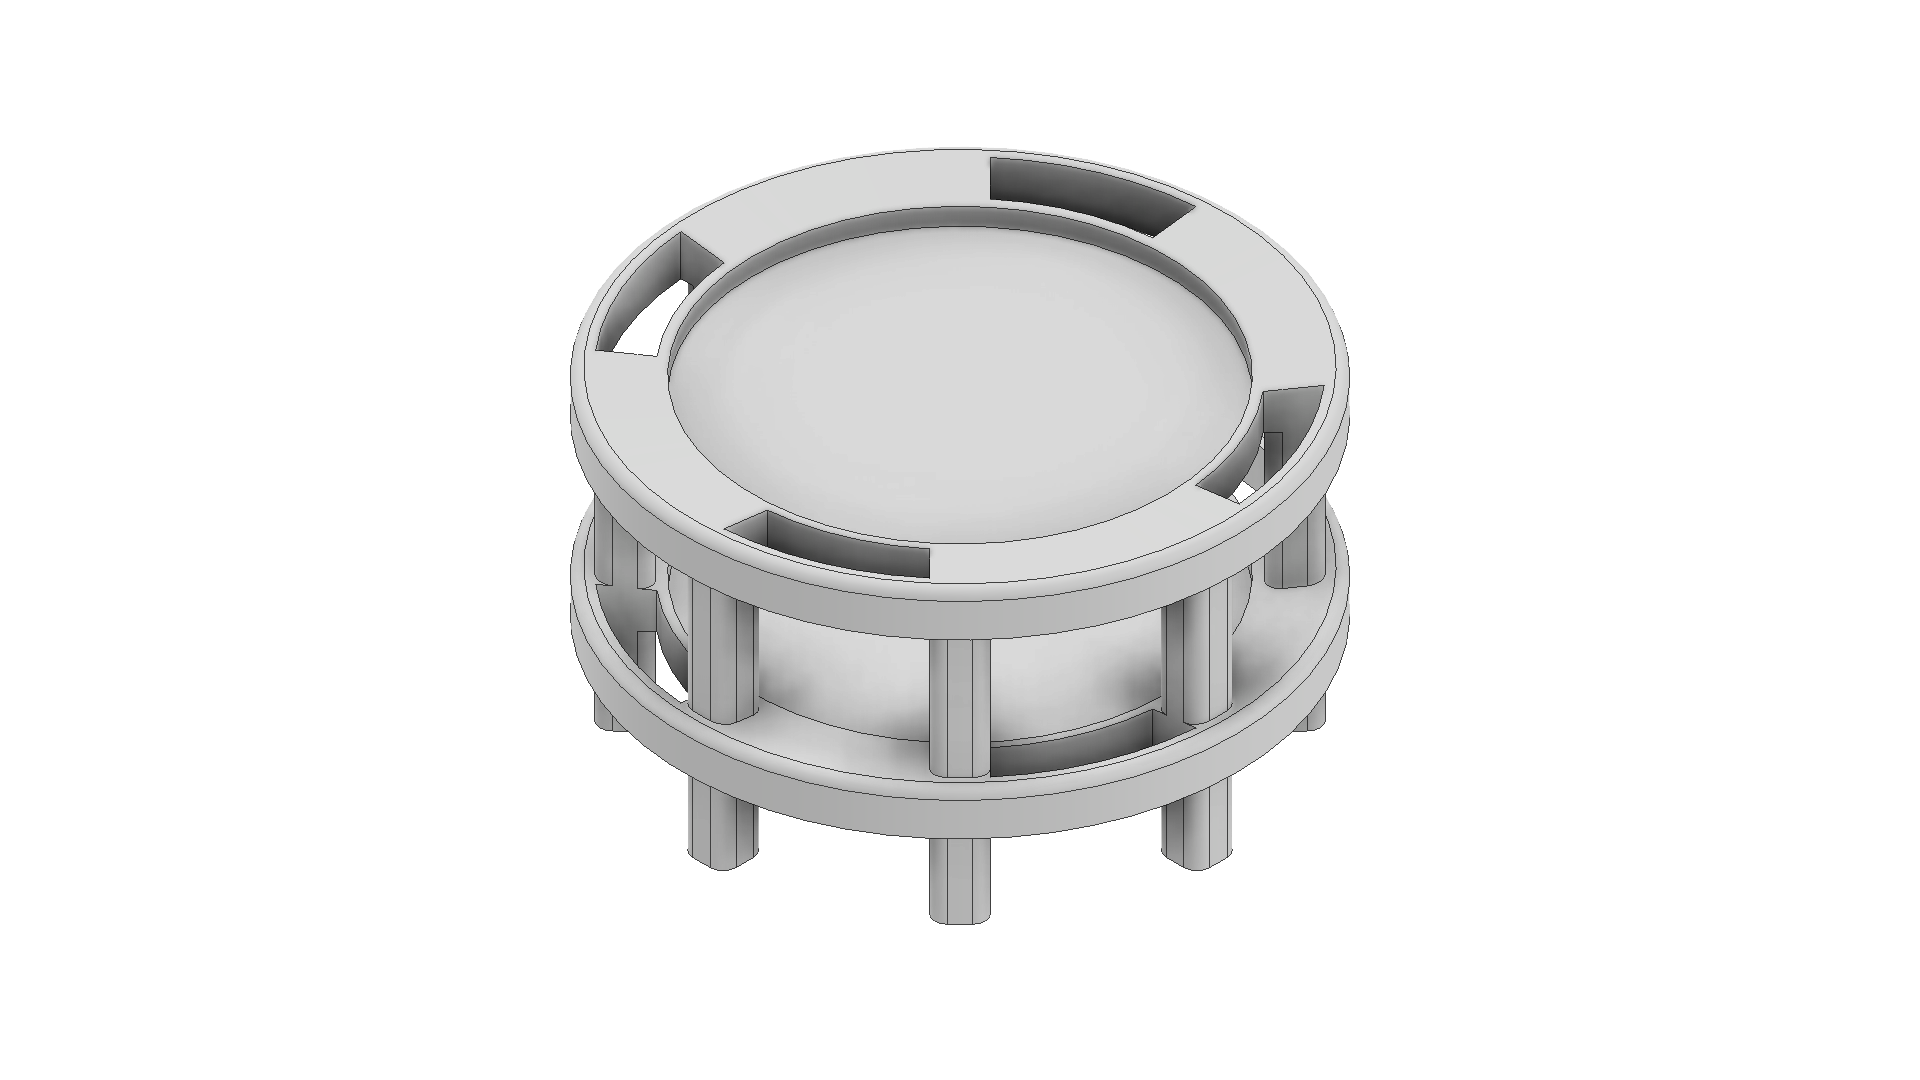
\includegraphics[
						width=\linewidth,
						height=70mm,
						keepaspectratio
					]{Resultados/Sistema/EvaporationSurface.png}
					\caption{Diseño sugerido para aumentar el área de evaporación dentro de la cámara}
					\label{fig:EvaporationSurface}
				\end{figure}
				
				Este submódulo consta de 2 entradas y 2 salidas.
				
				\begin{itemize}[columns=2]
					\item Entrada de agua caliente
					\item Entrada de aire de recirculación
					\item Salida de vapor caliente
					\item Salida de salmuera
				\end{itemize}
				
				\begin{center}
					En este módulo se monitorea la temperatura del agua.
				\end{center}
			
			\subsubsection{Intercambiador de calor}
			
				Este módulo tiene la función de enfriar el vapor caliente para condensar el agua destilada y a su vez inyectar ese calor al agua de mar entrante.
				
				\begin{figure}[H]
					\centering
					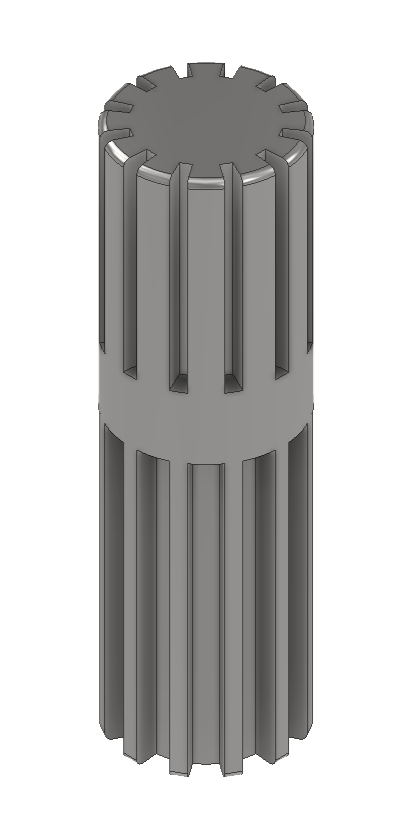
\includegraphics[
						width=\linewidth,
						height=70mm,
						keepaspectratio
					]{Resultados/Sistema/HeatExchanger.png}
					\caption{Diseño sugerido para el intercambiador de calor}
					\label{fig:HeatExchanger}
				\end{figure}
			
			\subsubsection{Módulo de concentración solar}
				
				Este módulo se divide en dos partes por cuestiones de ensamble y manufactura. La parte superior se encarga de soportar un cristal de borosilicato por el cual atraviesan los rayos solares. Este cristal permite mantener un mejor aislamiento térmico del recibidor solar así como evitar la exposición directa al ambiente.
				
				Por otra parte, en el submódulo inferior ocurre el intercambio de calor entre el recibidor solar y el agua. Esto se logra por medio de la conducción de calor entre el recibidor y una tubería de cobre. La elección de la tubería de cobre se dio debido a su alta conductividad térmica, flexibilidad, disponibilidad y costos, ya que en un inicio se planteó el uso de acero galvanizado y de acero inoxidable 316, sin embargo, como se mostrará en las simulaciones siguientes no resultaba buen conductor térmico además de ser difícilmente manufacturable; también se descartó el uso de tuberías de aluminio 5052 debido a su escaza disponibilidad.
				
				Este submódulo consta de 1 entrada y 1 salida.
				
				\begin{itemize}[columns=2]
					\item Entrada de agua fría
					\item Salida de agua caliente
				\end{itemize}
				
				\begin{center}
					En este módulo se monitorea la temperatura del recibidor solar.
				\end{center}
		
		\subsection{Simulaciones del sistema desalinizador}
			
			Se realizaron varias simulaciones de transferencia de calor con el fin de validar los diseños propuestos, los materiales seleccionados y el caudal propuesto durante el desarrollo experimental. A su vez, se realizaron simulaciones del flujo de aire en la cámara de evaporación con el fin de validar el diseño visto en la~\cref{fig:EvaporationSurface}.
			
			\subsubsection{Materiales y geometría}
			
				\textbf{Transferencia de calor}\par
			
				Con el fin de observar el desempeño de los materiales a utilizar para intercambiar calor con el recibidor solar, se simuló transferencia de calor con cobre, aluminio y acero inoxidable bajo condiciones favorables (Alta generación de calor). De estas simulaciones se concluyó que:
				
				\begin{enumerate}
					\item El acero inoxidable no proporciona una conducción suficiente de calor, ya que el recibidor empieza a sobrecalentarse mientras que el agua no adquiere la temperatura suficiente. Si se observa detenidamente la~\cref{fig:stainless-steel-heat-transfer} se observa que el agua se calienta cuando está más cerca del recibidor, sin embargo, el calor no llega a toda la tubería, por lo que esta se vuelve a enfriar una vez que se aleja del recibidor. Además, el recibidor comienza a sobrecalentarse al no deshacerse del calor, transfiriéndolo a los aislantes térmicos y los alrededores del recibidor. 
					\item El cobre es un buen candidato, ya que la tubería se calienta uniforme y rápidamente, además, el agua adquiere una temperatura poco menor que la del recibidor.
					
					\item El aluminio 5052 es un buen candidato, ya que la tubería se calienta rápidamente, sin embargo, incrementa la diferencia entre la temperatura del agua y la del recibidor en contraste con el cobre, sin mencionar que el agua se calienta de manera menos uniforme.
				\end{enumerate}
				
				\begin{figure}[H]
					\centering
					\begin{subfigure}[t]{\linewidth}
						\centering
						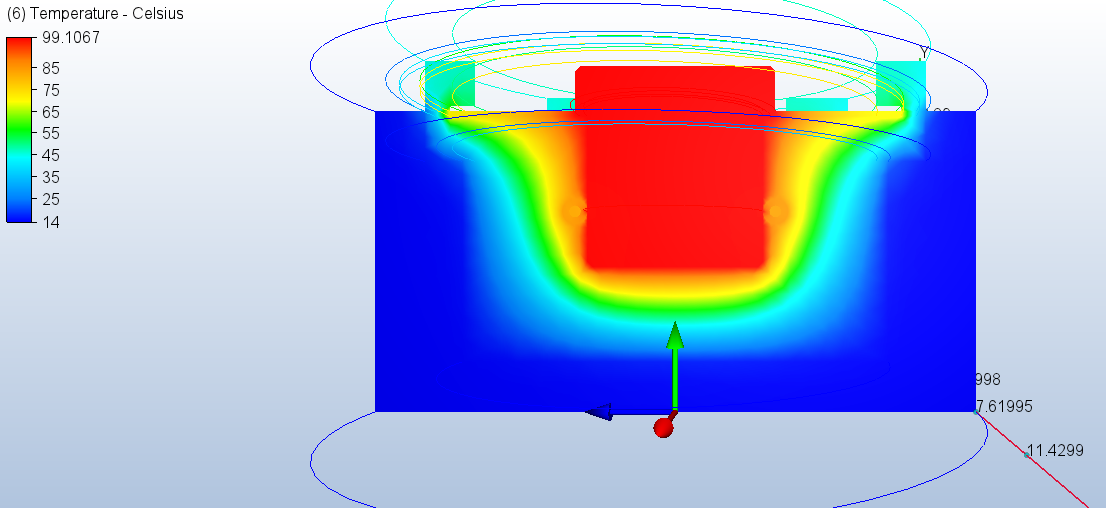
\includegraphics[
							width=\linewidth,
							height = 60mm,
							keepaspectratio
						]{Resultados/Simulaciones/50W-StainleesSteel-15C-9mlpm-middle.png}
						\caption{Corte en el centro del recibidor solar y su transferencia de calor hacia el acero inoxidable 316}
						\label{fig:50W-StainleesSteel-15C-9mlpm-middle}
					\end{subfigure}
				\end{figure}

				\begin{figure}[H]\ContinuedFloat
					\begin{subfigure}[t]{\linewidth}
						\centering
						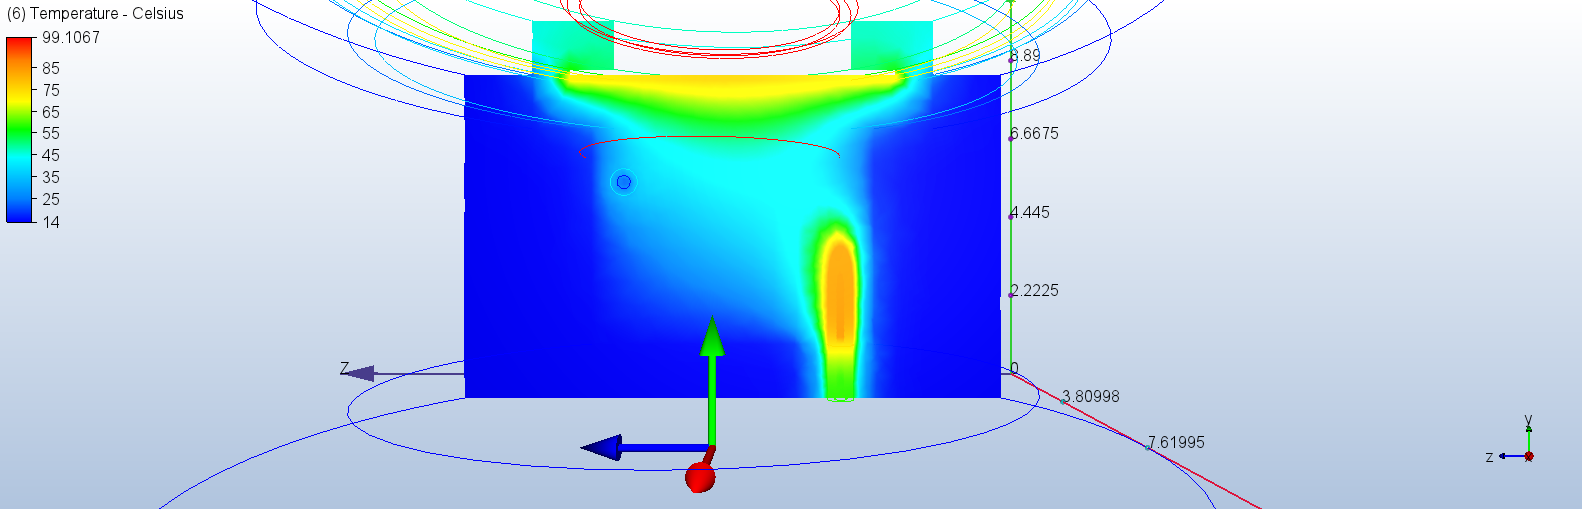
\includegraphics[
							width=\linewidth,
							height = 60mm,
							keepaspectratio
						]{Resultados/Simulaciones/50W-StainleesSteel-15C-9mlpm.png}
						\caption{Corte en la entrada y salida del agua de mar}
						\label{fig:50W-StainleesSteel-15C-9mlpm}
					\end{subfigure}
					\hfill
					\caption{Transferencia de calor en el acero inoxidable}
					\label{fig:stainless-steel-heat-transfer}
				\end{figure}
				
				\begin{figure}[H]
					\centering
					\begin{subfigure}[t]{\linewidth}
						\centering
						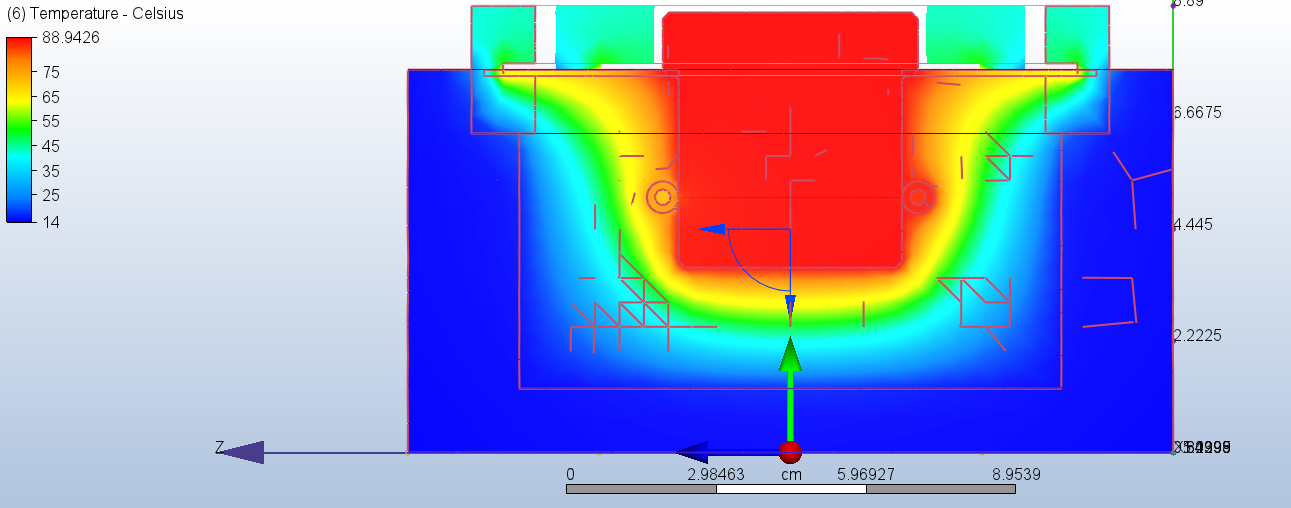
\includegraphics[
							width=\linewidth,
							height = 60mm,
							keepaspectratio
						]{Resultados/Simulaciones/50WCopper15C9mlpm-middle.png}
						\caption{Corte en el centro del recibidor solar y su transferencia de calor hacia el cobre}
						\label{fig:50WCopper15C9mlpm-middle}
					\end{subfigure}
				\end{figure}

				\begin{figure}[H]\ContinuedFloat
					\begin{subfigure}[t]{\linewidth}
						\centering
						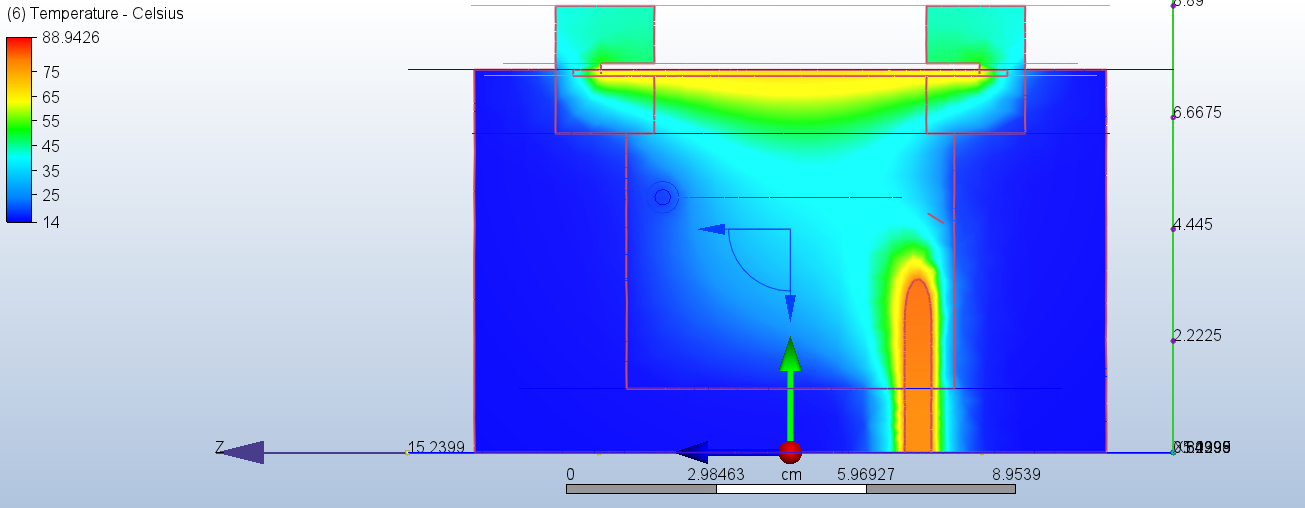
\includegraphics[
							width=\linewidth,
							height = 60mm,
							keepaspectratio
						]{Resultados/Simulaciones/50WCopper15C9mlpm.png}
						\caption{Corte en la entrada y salida del agua de mar}
						\label{fig:50WCopper15C9mlpm}
					\end{subfigure}
					\hfill
					\caption{Transferencia de calor en el cobre}
					\label{fig:copper-heat-transfer}
				\end{figure}
				
				\begin{figure}[H]
					\centering
					\begin{subfigure}[t]{\linewidth}
						\centering
						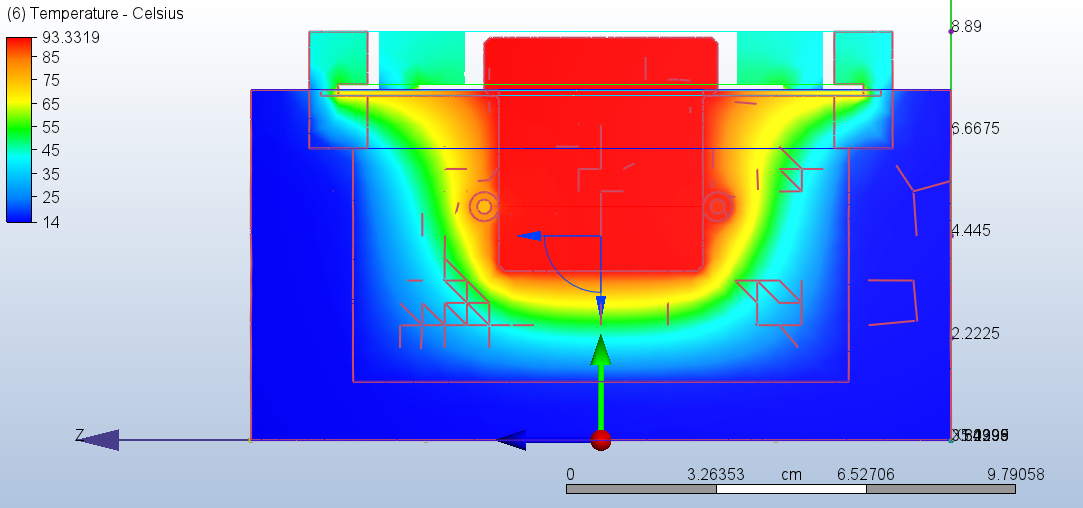
\includegraphics[
							width=\linewidth,
							height = 60mm,
							keepaspectratio
						]{Resultados/Simulaciones/50WAluminum15C9mlpm-middle.png}
						\caption{Corte en el centro del recibidor solar y su transferencia de calor hacia el aluminio}
						\label{fig:50WAluminum15C9mlpm-middle}
					\end{subfigure}
				\end{figure}

				\begin{figure}[H]\ContinuedFloat
					\begin{subfigure}[t]{\linewidth}
						\centering
						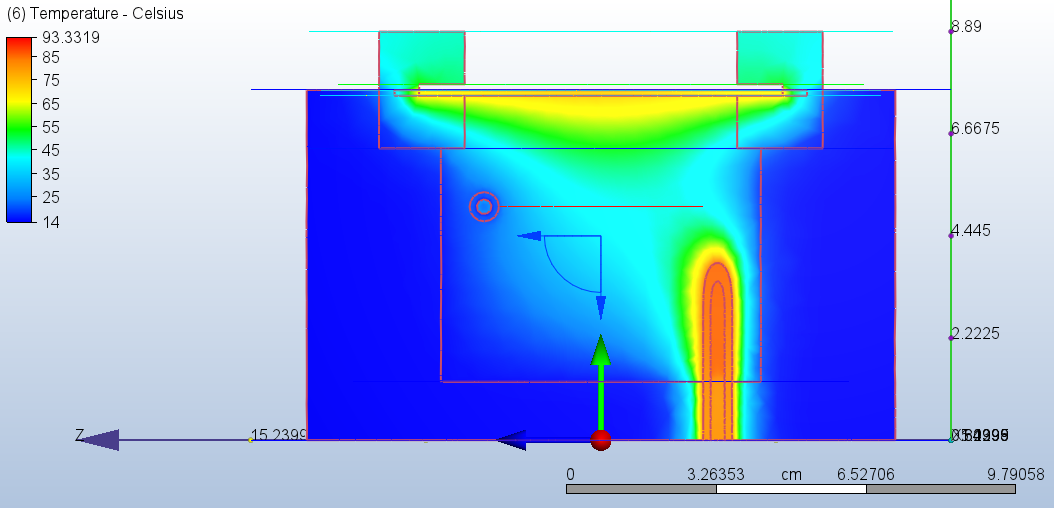
\includegraphics[
							width=\linewidth,
							height = 60mm,
							keepaspectratio
						]{Resultados/Simulaciones/50WAluminum15C9mlpm.png}
						\caption{Corte en la entrada y salida del agua de mar}
						\label{fig:50WAluminum15C9mlpm}
					\end{subfigure}
					\hfill
					\caption{Transferencia de calor en el aluminio}
					\label{fig:aluminum-heat-transfer}
				\end{figure}
				
				Se simularon 300 segundos de transferencia de calor de los tres materiales bajo las condiciones halladas en el desarrollo experimental en lugar de buscar la convergencia, ya que esto requeriría un tiempo mucho mayor y observando el comportamiento de la temperatura del recibidor se concluyó que la información proporcionada fue suficiente para llegar a una conjetura.
				
				De las simulaciones se observó que la temperatura del recibidor solar crecía más rápidamente que la temperatura del agua de salida; en cambio, el cobre y el aluminio tuvieron mejores respuestas.
				
				\textit{Producto de estas simulaciones}
				
				Las anteriores simulaciones ayudaron a comprender un poco más la respuesta del sistema y con base en ello se tomaron las siguientes decisiones.
				
				\begin{itemize}
					\item Se descartó el uso de acero inoxidable como material para la tubería
					\item Se aceptó el uso de aluminio 5052 como material para la tubería pero se identificaron ciertas limitaciones en contraste con el cobre como menor ductibilidad, menor transferencia de calor pero mayor resistencia a la corrosión.
					\item Los criterios de manufacturabilidad cambiaron cuando se eligió el cobre como material para la tubería. Como resultado, se propuso un nuevo diseño para mejorar la homogeneidad de la temperatura del agua, esto se muestra en la~\cref{fig:FuzzyUniverse}.
				\end{itemize}
				
				
				\textbf{Flujo de aire en la cámara de evaporación}\par
			
				La superficie de evaporación vista en la~\cref{fig:EvaporationSurface} incrementa a más del doble la superficie de evaporación y no disminuye sustancialmente el flujo de aire dentro de la cámara como se observa en la~\cref{fig:AirflowInEvaporationChamber}, por lo cual se justifica parcialmente su incorporación al desalinizador dado que falta evaluar su influencia en la acumulación de sales dentro de la cámara.
				
				\begin{figure}[H]
					\centering
					\begin{subfigure}[t]{0.45\linewidth}
						\centering
						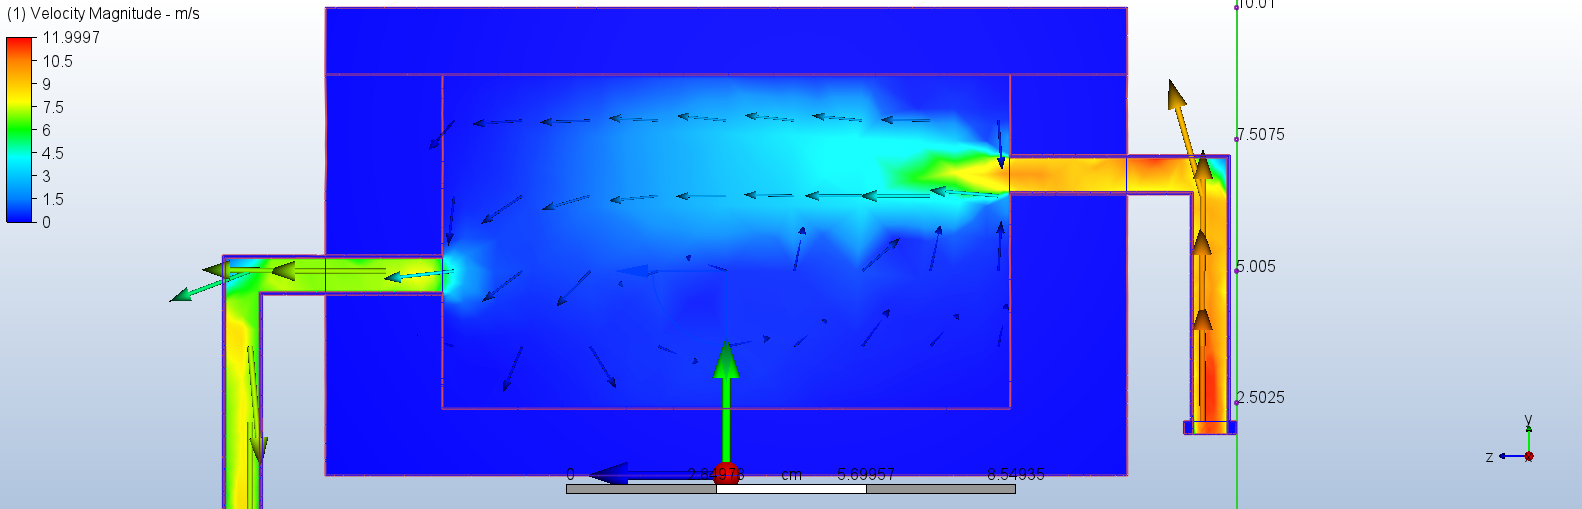
\includegraphics[
							width=\linewidth,
							height = 60mm,
							keepaspectratio
						]{Resultados/Simulaciones/AirflowWithoutEvaporationSurface.png}
						\caption{Flujo de aire sin superficie de evaporación}
						\label{fig:AirflowWithoutEvaporationSurface}
					\end{subfigure}
					\hfill
					\begin{subfigure}[t]{0.45\linewidth}
						\centering
						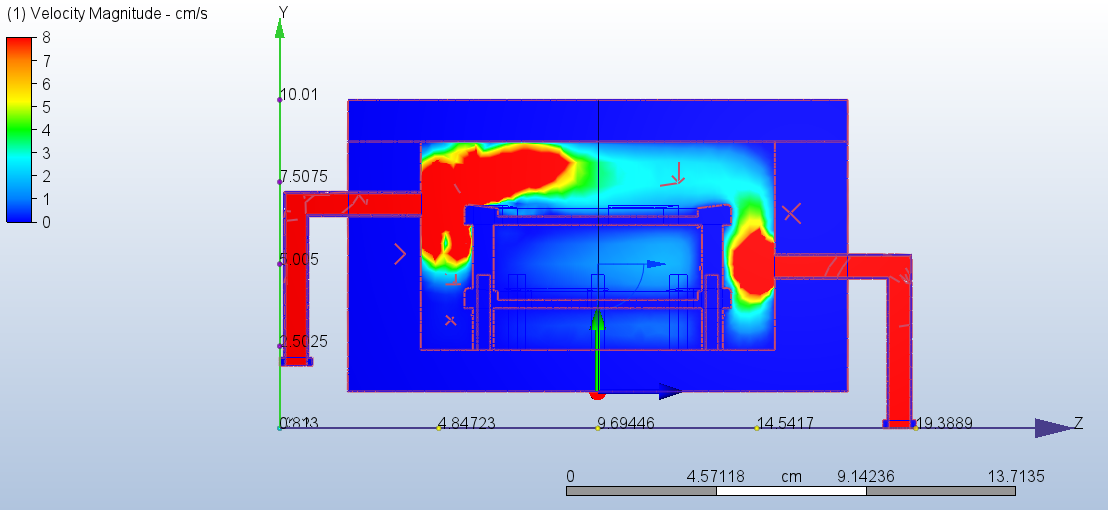
\includegraphics[
							width=\linewidth,
							height = 60mm,
							keepaspectratio
						]{Resultados/Simulaciones/AirflowWithEvaporationSurface.png}
						\caption{Flujo de aire con superficie de evaporación}
						\label{fig:AirflowWithEvaporationSurface}
					\end{subfigure}
					\caption{Flujo de aire en la cámara de evaporación}
					\label{fig:AirflowInEvaporationChamber}
				\end{figure}
				
	\section{Control del sistema}
	
		\subsection{Sensores y componentes, calibración y caracterización}\label{subsec:calibración}
		
			A continuación se detalla el proceso de ajuste y caracterización de los sensores y la bomba que regula el flujo de agua, estas calibraciones resultan indispensables para el correcto funcionamiento del método de control.
			
			\textbf{Termistores}\par
			
			Para caracterizar los termistores se refirió a un set de datos que reflejan la respuesta óhmica al aplicarse cierta temperatura; el código visto en~\cref{ch:steinhart-code} permite hallar los coeficientes de Steinhart-Hart para este modelo.
			
			Se halló que:
			
			\begin{itemize}[columns=3]
				\item A = \num{1.12866e-3}
				\item B = \num{2.3422e-4}
				\item C = \num{8.7159e-8}
			\end{itemize}
			
			\textbf{EZO-PMP}\par
			
			La bomba peristáltica EZO-PMP permite una calibración manual, para ello se recreó la configuración vista en la~\cref{fig:Calibración-bomba}
			
			\begin{figure}[H]
				\centering
				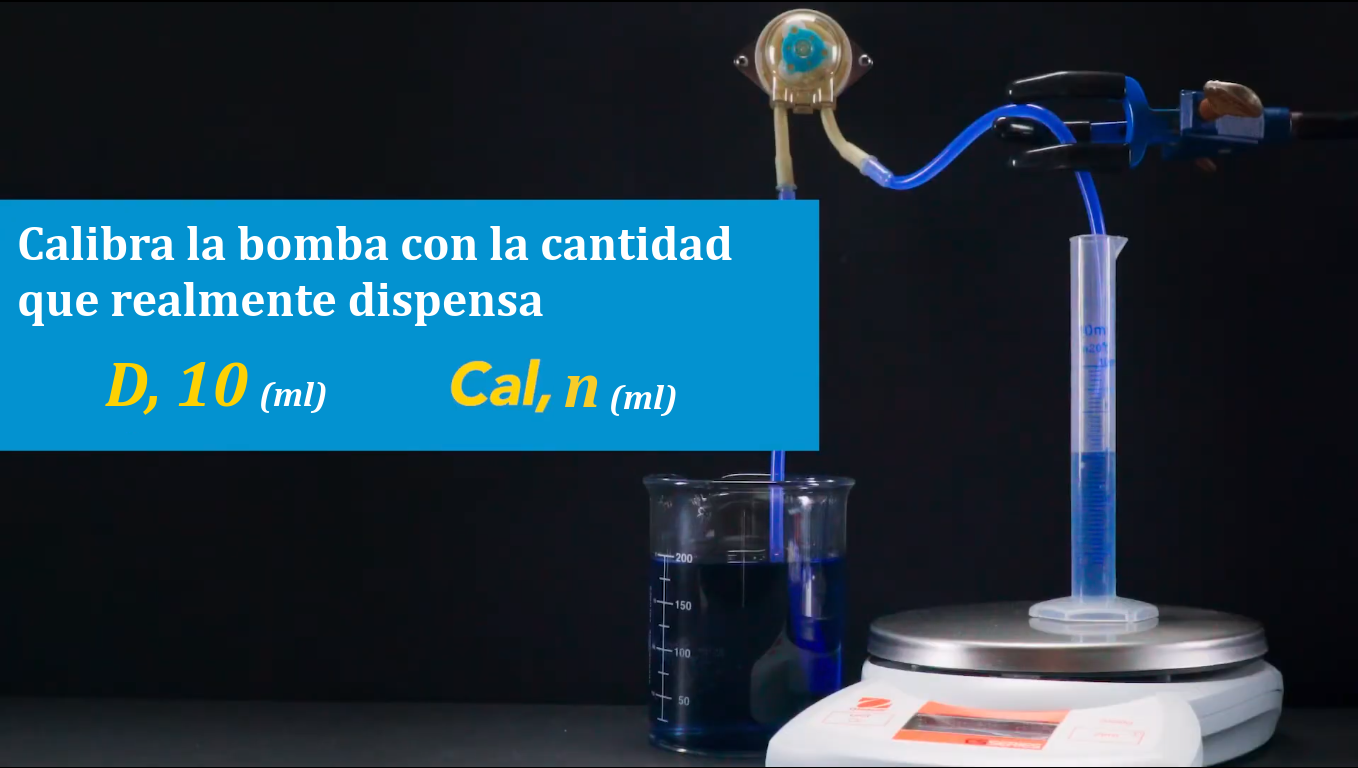
\includegraphics[
					width=\linewidth,
					height=65mm,
					keepaspectratio
				]{Resultados/Control/PumpCalibration.png}
				\caption{Arreglo para la calibración de la bomba EZO-PMP}
				\floatfoot{Imagen adaptada de \cite{atlas_scientific_llc_ezo-pmp_2020}}
				\label{fig:Calibración-bomba}
			\end{figure}
			
		\subsection{Selección del método de control}
	
			Considerando el tamaño del sistema y las diferentes funciones que debe atender, se decidió dividir el control en dos partes, la primera regula el flujo de agua que pasa por el recibidor solar y la última se centra en abastecer y vaciar el sistema, es decir, se encarga de vaciar el agua condensada, la salmuera y restablecer los niveles de agua de mar. Debido a la naturaleza más simple de la segunda parte del control, se proporcionará una explicación breve al final. Por el momento, se justificará la selección del método de control propuesto.
			
		
			En la primera etapa, se llevaron a cabo estudios comparativos para evaluar distintos métodos de control, analizando sus ventajas y desventajas. Tras este análisis, se llegó a la conclusión de que el método de control difuso se acoplaba mejor a las necesidades del sistema ya que:
			
			\begin{itemize}
				\item El modelo de contro difuso permite hacer razonamientos para evaluar el grado de certidumbre de una afirmación en vez de limitarse a una lógica binaria donde se producen saltos de una afirmación a otra.
				\item Permite crear un modelo de control basado en reglas fácilmente interpretables
				\item No requiere un modelo matemático u aproximación numérica del proceso, sino, en conocimiento empírico, lo cual es muy beneficioso, ya que tanto el proceso de evaporación como el de ebullición es un fenómeno muy complejo y difícilmente modelable.
				\item Permite tomar decisiones de conocimientos y datos inexactos de forma similar al razonamiento humano
			\end{itemize}		
		
		\subsection{Modelo y reglas del control difuso}
				
			Se decidió restringir las variables difusas exclusivamente a la temperatura del agua de entrada y la del recibidor solar. Esta decisión se tomó considerando que un gran número de variables podría aumentar exponencialmente la complejidad del algoritmo y las reglas.
			
			Con el fin de definir las funciones de membresía se se estudió la respuesta del sistema  variando el caudal, la temperatura del agua entrante y el calor capturado por el concentrador solar. Mediante simulaciones se pudo delimitar el universo de discurso de las variables difusas y comprender su impacto en el modelo.	En la~\cref{fig:FuzzyUniverse} se muestra brevemente evidencia de las diferentes simulaciones hechas.
								
			\begin{figure}[H]
				\centering
				\includegraphics[
					width=\linewidth,
					height = 60mm,
					keepaspectratio
				]{Resultados/Simulaciones/FuzzyUniverse.png}
				\caption{Captura de pantalla de Autodesk CFD mostrando una vista general de las simulaciones realizadas}
				\label{fig:FuzzyUniverse}
			\end{figure}
			
			Durante la corrida de las simulaciones se observó que:
			
			\begin{enumerate}
				\item En esta nueva geometría de la tubería de cobre, el agua de salida adquiere prácticamente la temperatura del agua solar una vez se estabiliza el intercambio de calor. Cabe resaltar que esta temperatura y la temperatura del agua a evaporar son distintas.
				\item La variación del flujo de agua tiene el mayor impacto en el sistema; un cambio repentino en el flujo de agua tiene un impacto significativo en la temperatura del agua de salida.
				\item La variación de la temperatura del agua entrante tiene un impacto notable en la temperatura del agua de salida, aunque es necesario un rango amplio para notar esta diferencia.
			\end{enumerate} 
						
			Se propuso entonces utilizar una función de membresía triangular para el caudal, ya que representa con mayor precisión los cambios bruscos que produce en la respuesta del sistema. En cuanto a la temperatura del receptor solar, se propuso una función gaussiana debido a que se ajusta más al comportamiento observado.
			
			Posteriormente se definieron las variables lingüísticas y sus respectivas membresías. En las dos variables difusas de entrada, se establecieron cinco variables lingüísticas cada una, mientras que en la variable difusa de salida se definieron seis variables lingüísticas. Estas membresías y sus respectivos rangos son visibles en las~\cref{fig:var-membership-functions,fig:FlowVelocity}.
			
			\begin{figure}[H]
				\centering
				\begin{subfigure}[t]{0.45\linewidth}
					\centering
					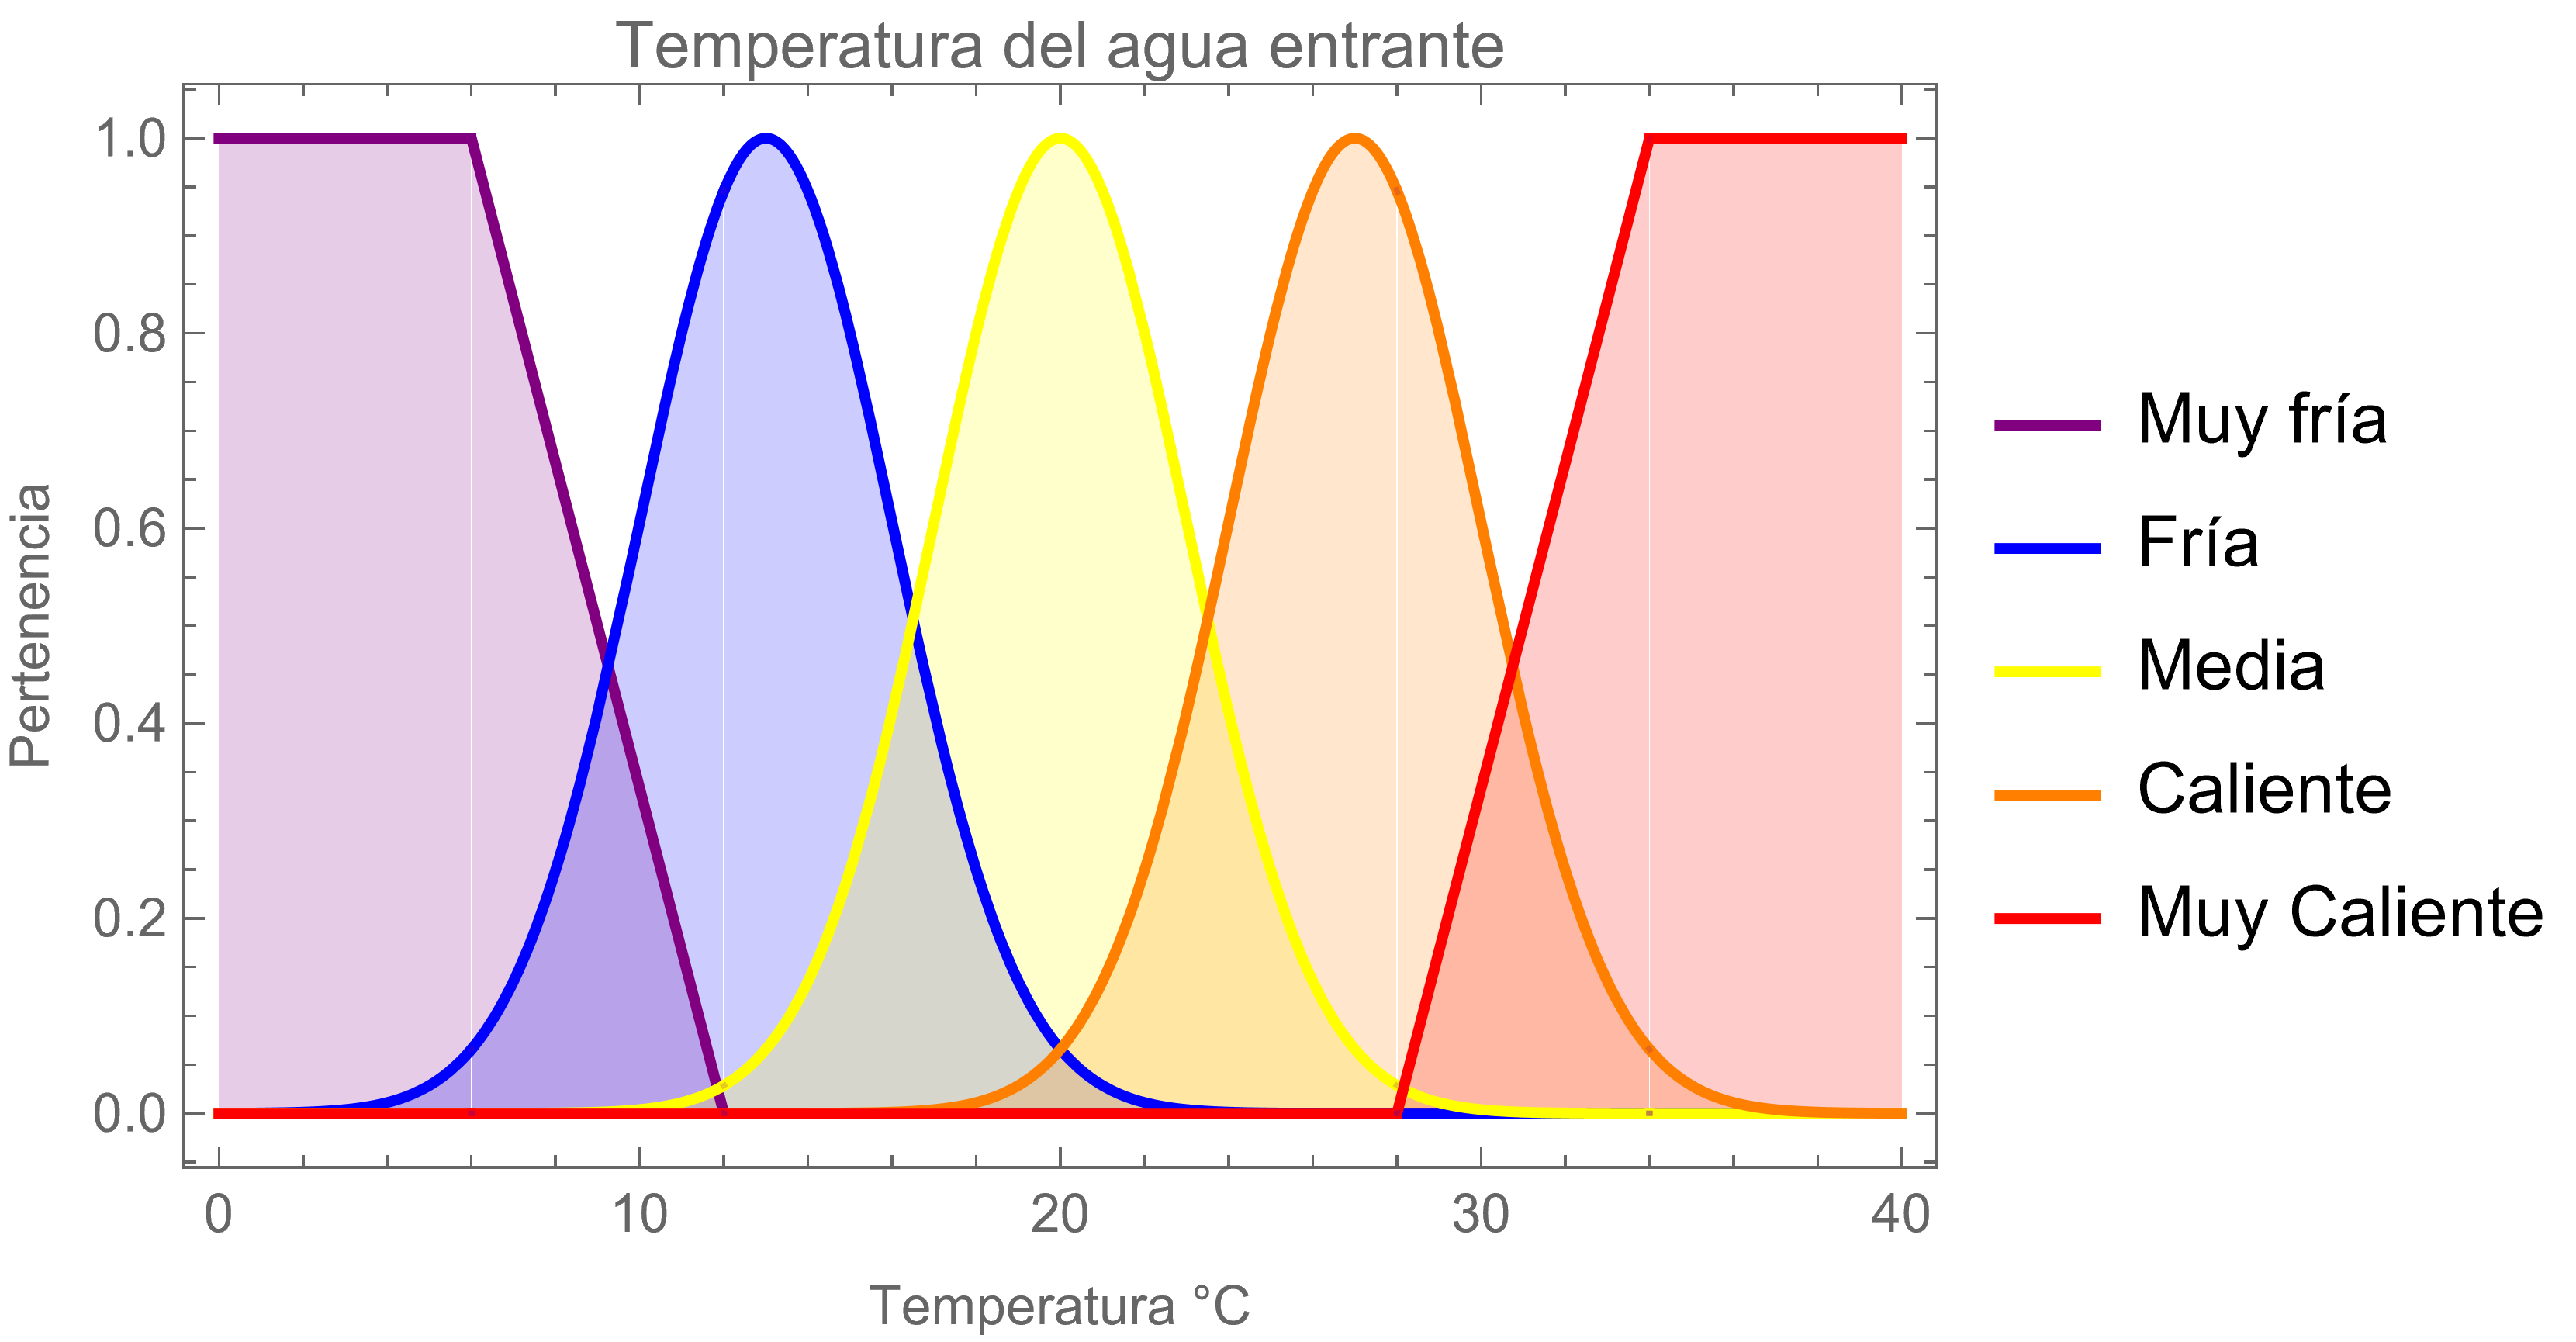
\includegraphics[
						width=\linewidth,
						height = 60mm,
						keepaspectratio
					]{Resultados/Control/SeawaterTemperature.png}
					\caption{Funciones de membresía de la temperatura del agua de mar entrante}
					\label{fig:SeawaterTemperature}
				\end{subfigure}
				\hfill
				\begin{subfigure}[t]{0.45\linewidth}
					\centering
					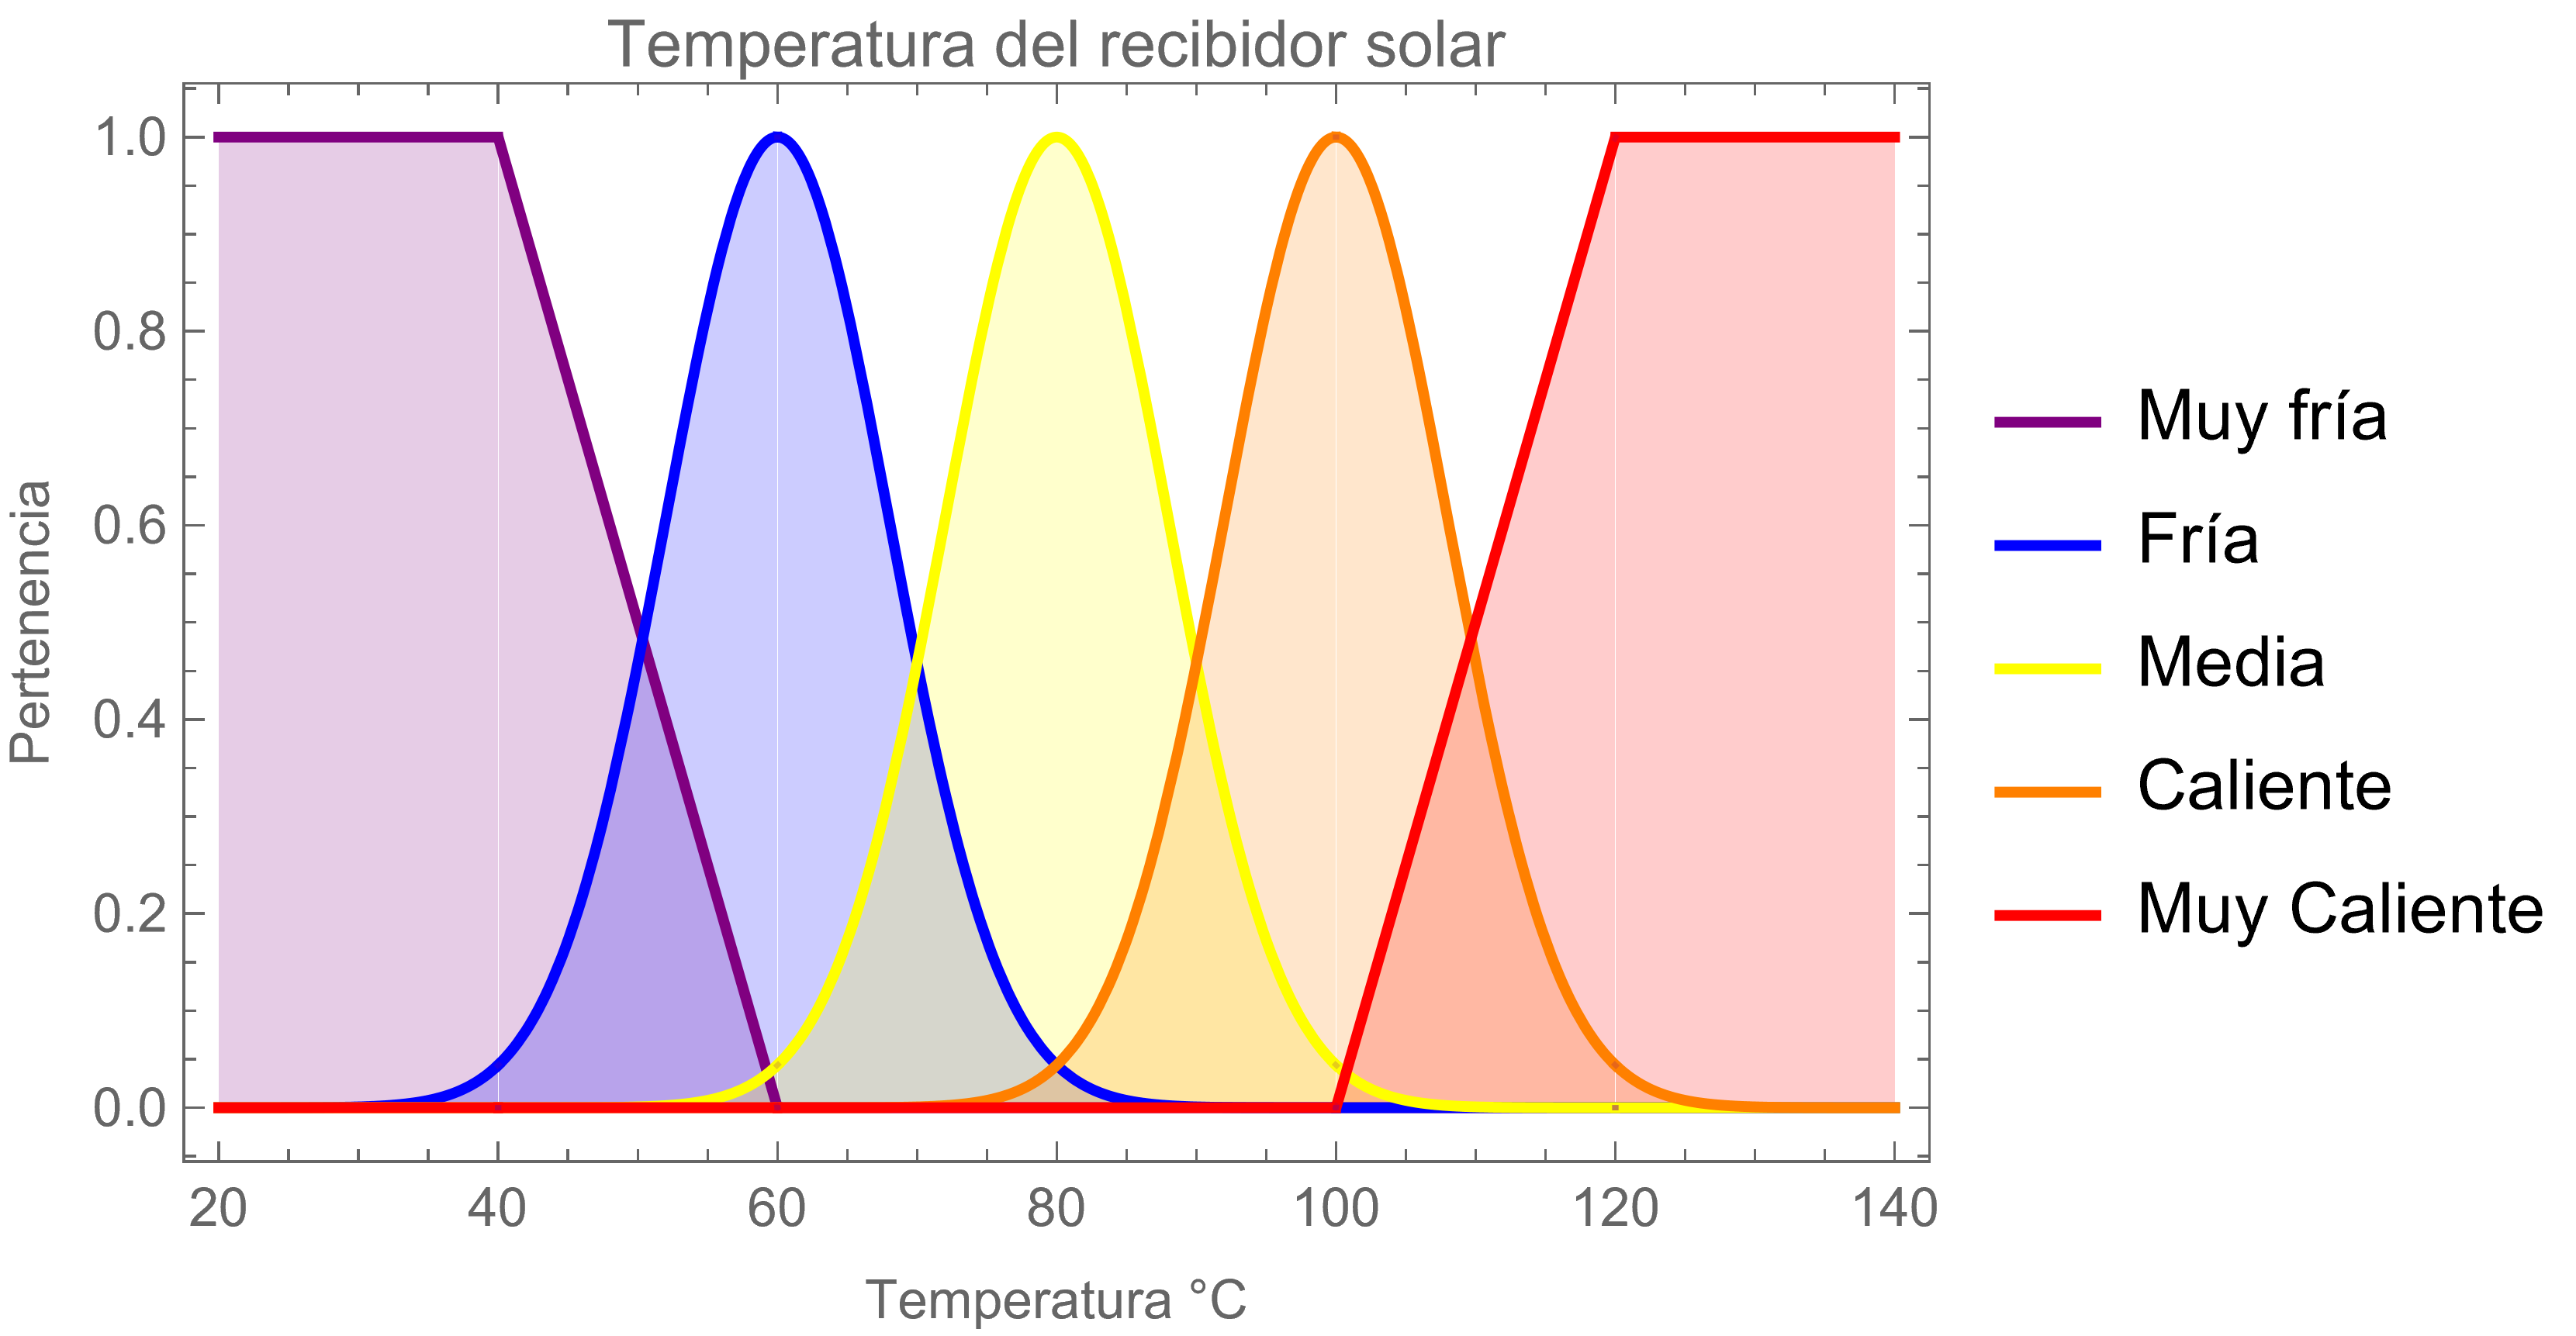
\includegraphics[
						width=\linewidth,
						height = 60mm,
						keepaspectratio
					]{Resultados/Control/SolarReceiverTemperature.png}
					\caption{Funciones de membresía de la temperatura del recibidor solar}
					\label{fig:SolarReceiverTemperature}
				\end{subfigure}
				\caption{Funciones de membresía de las variables difusas de entrada}
				\label{fig:var-membership-functions}
			\end{figure}
			
			\begin{figure}[H]
				\centering
				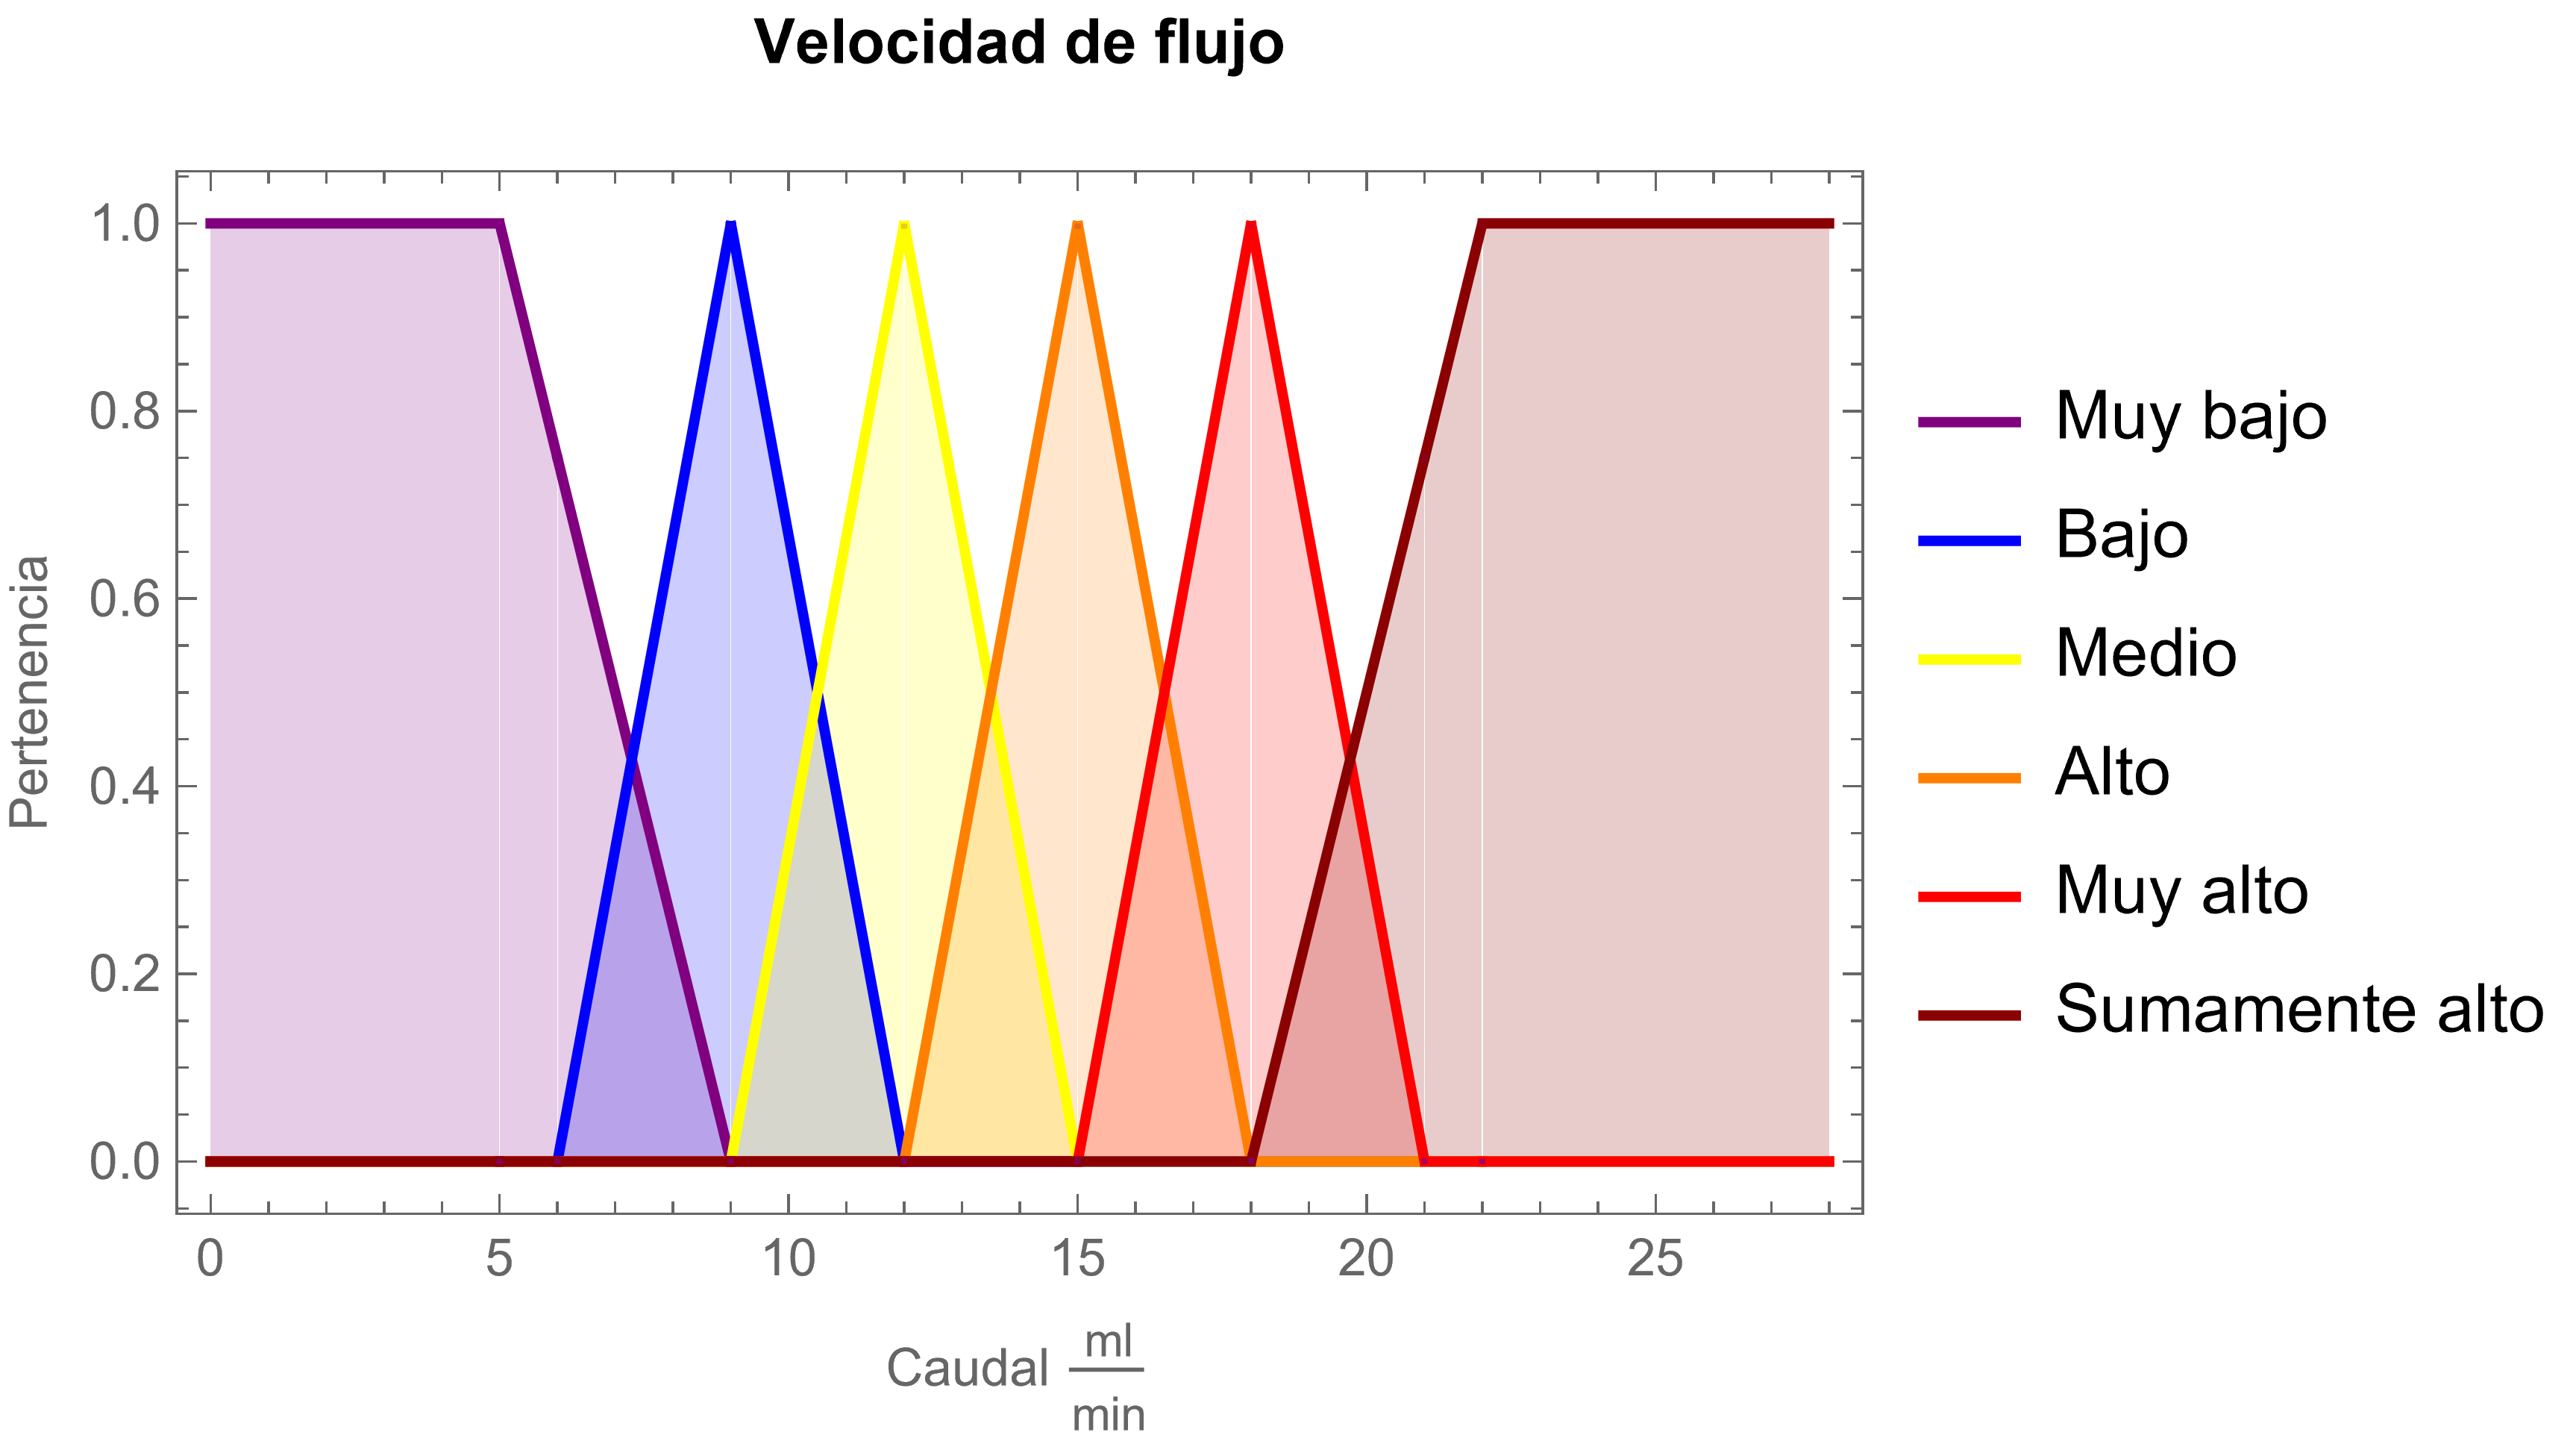
\includegraphics[
					width=\linewidth,
					height=65mm,
					keepaspectratio
				]{Resultados/Control/FlowVelocity.png}
				\caption{Funciones de membresía de la respuesta difusa.}
				\label{fig:FlowVelocity}
			\end{figure}
			
			Una vez llegado a este punto se definieron las reglas que rigen el sistema difuso. Para leerse con mayor facilidad se dividieron en bloques.
			
			\textit{Si la temperatura del recibidor solar es muy baja:}\par
			
			\begin{itemize}
				\item El caudal es nulo en todos los casos.
			\end{itemize}
			
			\textit{Si la temperatura del recibidor solar es baja:}\par
			\begin{itemize}
				\item Si la temperatura del recibidor solar es baja y además no es muy baja, y la temperatura del agua de entrada es muy alta, el caudal es medio.
				\item Si la temperatura del recibidor solar es baja y además no es muy baja, y la temperatura del agua de entrada es alta, el caudal es bajo.
				\item Si la temperatura del recibidor solar es baja y además no es muy baja, y la temperatura del agua de entrada es media pero no es baja, el caudal es muy bajo.
				\item Si la temperatura del recibidor solar es baja y además no es muy baja, y la temperatura del agua de entrada es muy baja o baja, el caudal es nulo.
			\end{itemize}
			
			\textit{Si la temperatura del recibidor solar es media:}\par
			\begin{itemize}
				\item Si la temperatura del recibidor solar es media y la temperatura del agua de entrada es alta o muy alta, el caudal es alto.
				\item Si la temperatura del recibidor solar es media y la temperatura del agua de entrada es media, el caudal es medio.
				\item Si la temperatura del recibidor solar es media y la temperatura del agua de entrada es baja, el caudal es bajo.
				\item Si la temperatura del recibidor solar es media y la temperatura del agua de entrada es muy baja, el caudal es muy bajo.
				
			\end{itemize}
			
			\textit{Si la temperatura del recibidor solar es alta:}\par
			\begin{itemize}
				\item Si la temperatura del recibidor solar es alta y la temperatura del agua de entrada es alta o muy alta, el caudal es muy alto
				\item Si la temperatura del recibidor solar es alta y la temperatura del agua de entrada es media, el caudal es alto.
				\item Si la temperatura del recibidor solar es alta y la temperatura del agua de entrada es baja, el caudal es medio.
				\item Si la temperatura del recibidor solar es alta y la temperatura del agua de entrada es muy baja, el caudal es bajo.
			\end{itemize}
			
			\textit{Si la temperatura del recibidor solar es muy alta:}\par
			\begin{itemize}
				\item Si la temperatura del recibidor solar es muy alta, y la temperatura del agua de entrada es muy alta el caudal es sumamente alto
				\item Si la temperatura del recibidor solar es muy alta y la temperatura del agua de entrada es alta, el caudal es muy alto
				\item Si la temperatura del recibidor solar es muy alta y la temperatura del agua de entrada es media, el caudal es alto
				\item Si la temperatura del recibidor solar es muy alta y la temperatura del agua de entrada es baja, el caudal es medio
				\item Si la temperatura del recibidor solar es muy alta y la temperatura del agua de entrada es muy baja, el caudal es bajo
			\end{itemize}
			
			Este conjunto de reglas tienen como objetivo tratar de mantener la temperatura del agua entre \qtyrange{62.5}{67.5}{\degreeCelsius} con el fin de evitar daños en los componentes eléctricos. Aunque se observó que sería un caso improbable, se decidió agregar una función protectora que aumenta el caudal al máximo si la temperatura del agua a evaporar se acerca peligrosamente a los \qty{70}{\degreeCelsius} (límite de operación de los componentes eléctricos seleccionados).
		
		\subsection{Automatización del vaciado y llenado de los módulos}
			
			Como se explicó anteriormente, esta segunda parte del control se encarga de administrar los volúmenes de agua dentro del ``Módulo de reaprovechamiento térmico y bombeo''.
			
			Para el contenedor de agua de mar, se usa un sensor de nivel para saber cuándo es necesario suministrar más agua al contenedor. Caso contrario, en el contenedor de agua destilada, se usa para saber cuándo es necesario vaciarlo. En el caso de la cámara de evaporación, se usa el sensor de temperatura y el estado del sistema de control difuso para saber si hay salmuera en la cámara. Si la temperatura de la salmuera baja de los \qty{40}{\degreeCelsius} o han transcurrido 2 horas de operación, se vacía la salmuera.

	
	\section{Integración al seguidor solar}
		
		Para integrar el desalinizador al seguidor solar, se construyeron dos estructuras, la primera es marco que soporta la lente, la altura de colocación de la lente se calculó mediante la ley de Snell y trigonometría siguiendo el arreglo mostrado en la~\cref{fig:DiagramaRayos}.
		
		De los cálculos hechos, se obtuvo una altura al punto focal de \qty{362.45}{\mm}. A eso se le sumó la altura del recibidor solar con respecto al módulo de concentración solar dando que la altura mínima del marco es de \qty{442.50}{\mm}.
		
		\begin{figure}[H]
			\centering
			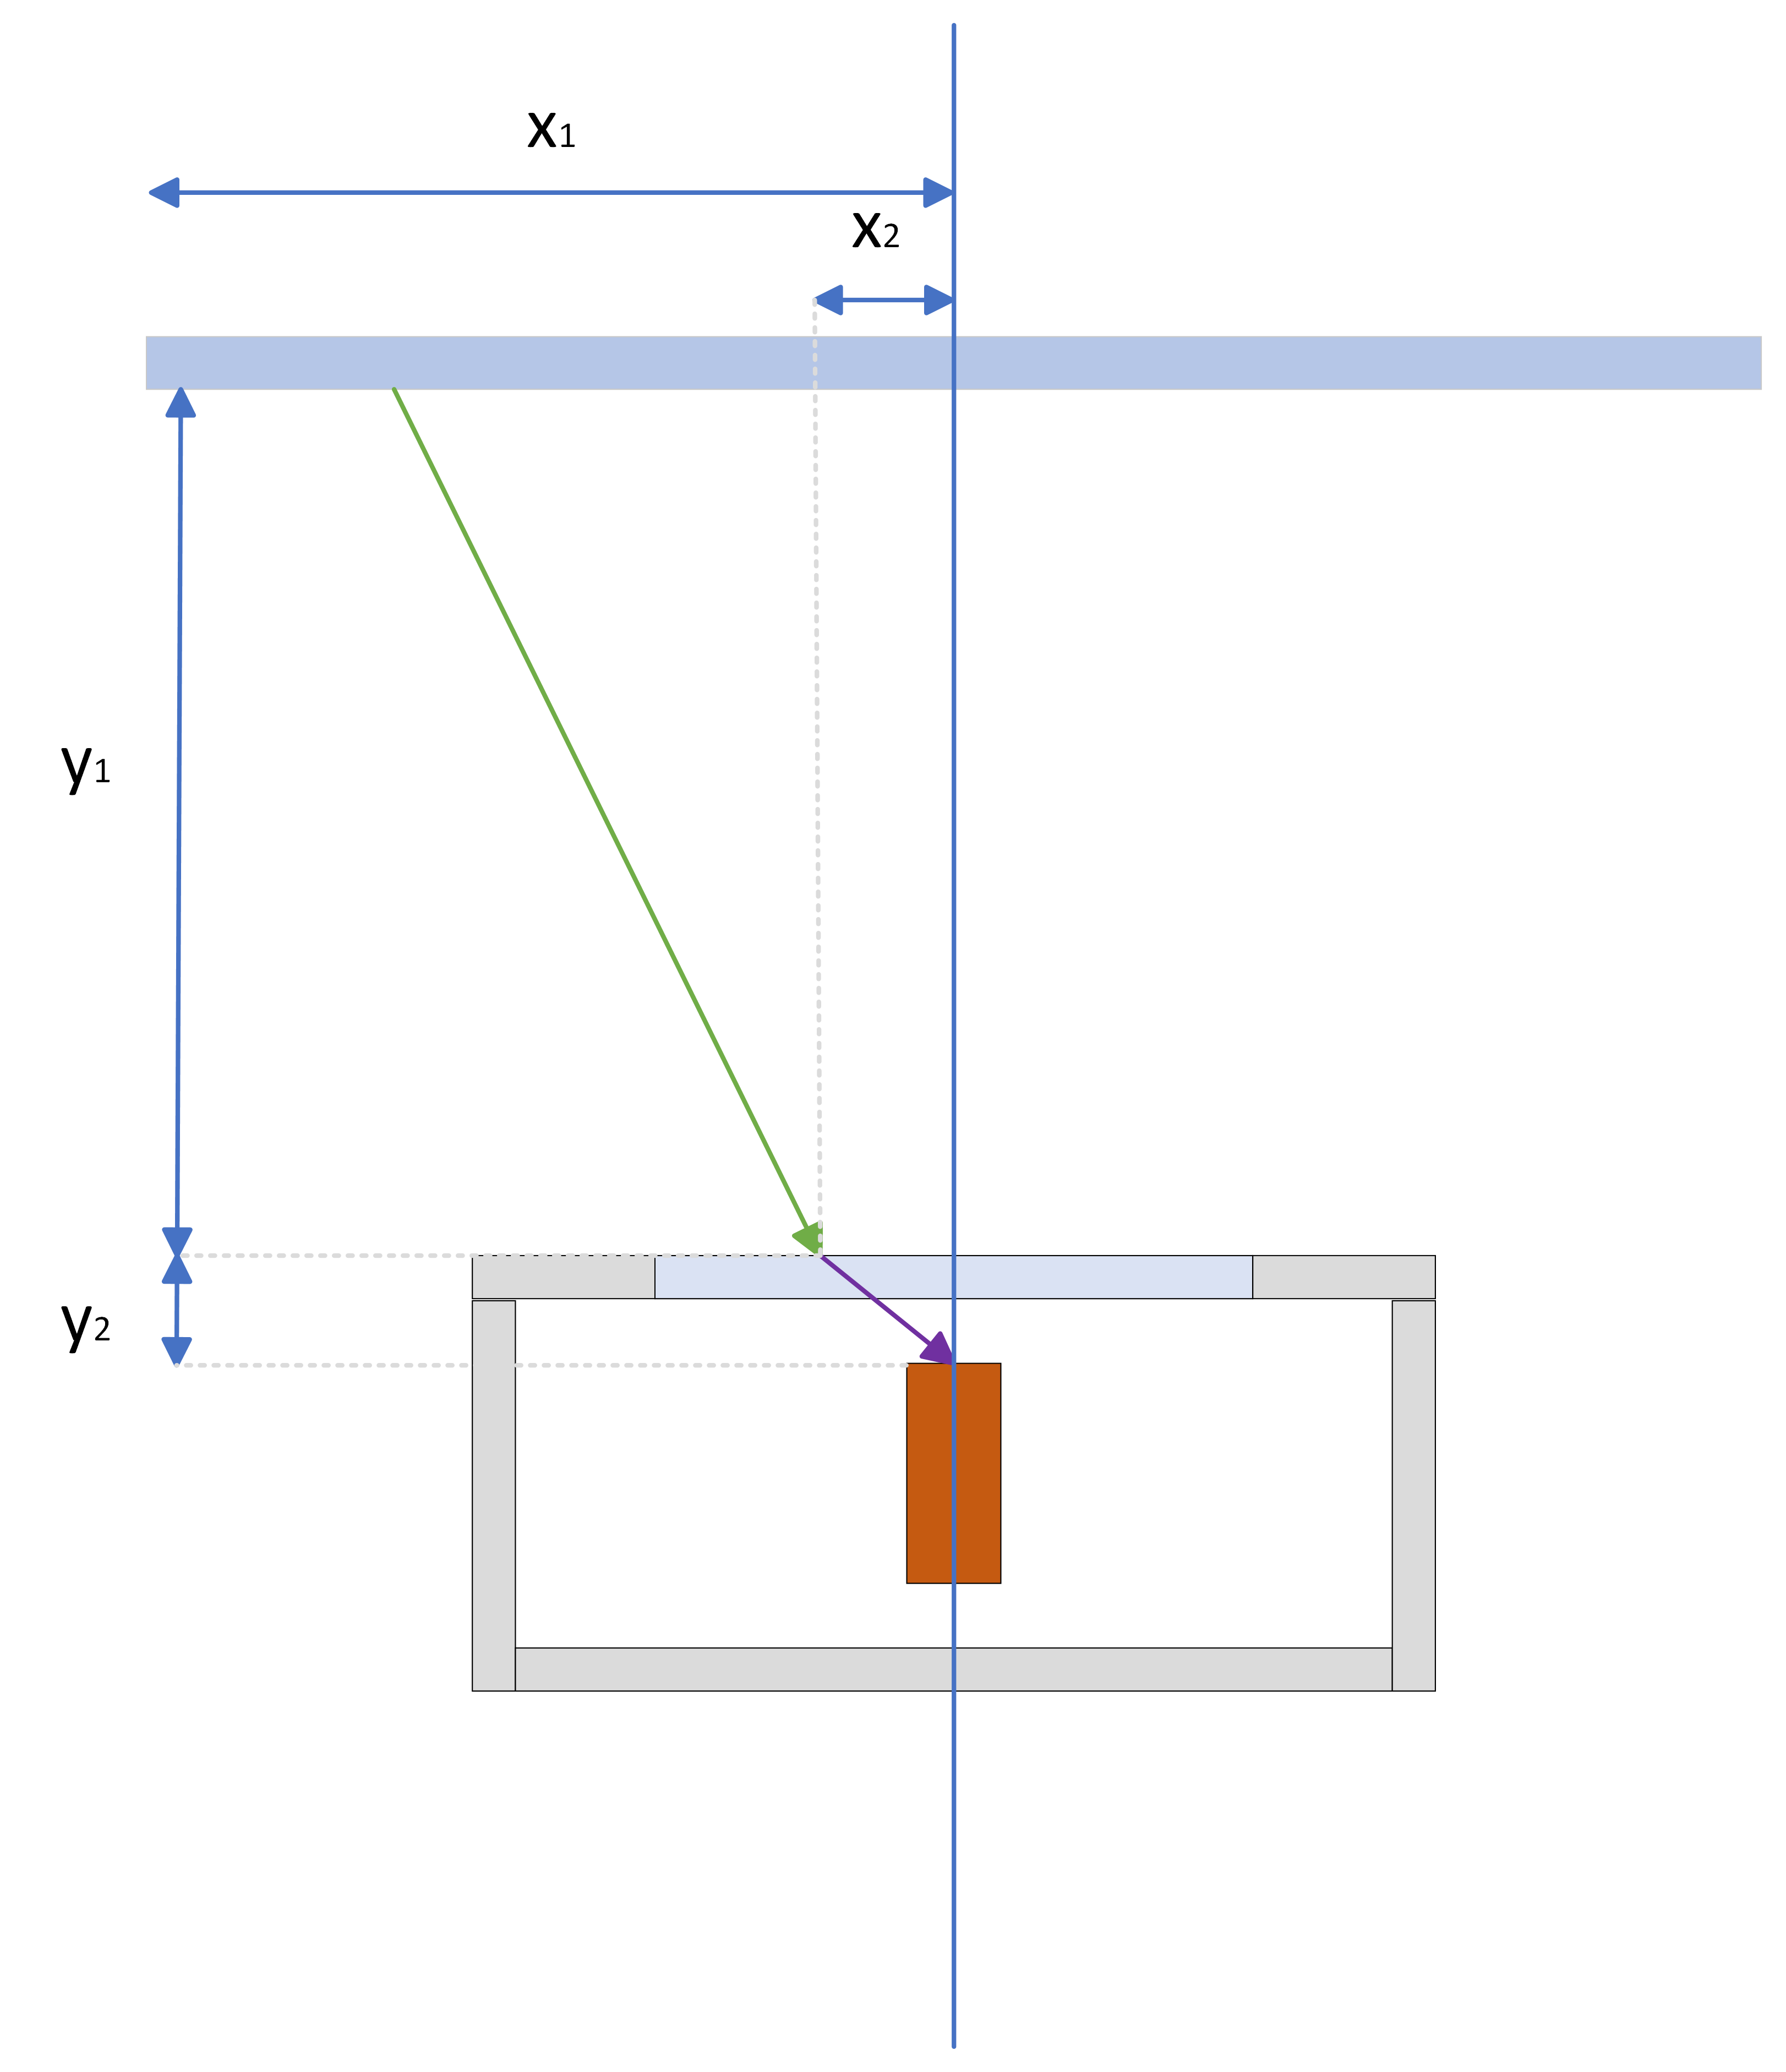
\includegraphics[
				width=\linewidth,
				height=65mm,
				keepaspectratio
			]{Resultados/Integración/DiagramaRayos.png}
			\caption{Trazado de rayos que permiten calcular la altura de la lente con respecto al punto focal.}
			\label{fig:DiagramaRayos}
		\end{figure}
		
		La segunda estructura (\cref{fig:DiagramaRayos}) es una base sobre la que reposa la base de agua.
		
		\begin{figure}[H]
			\centering
			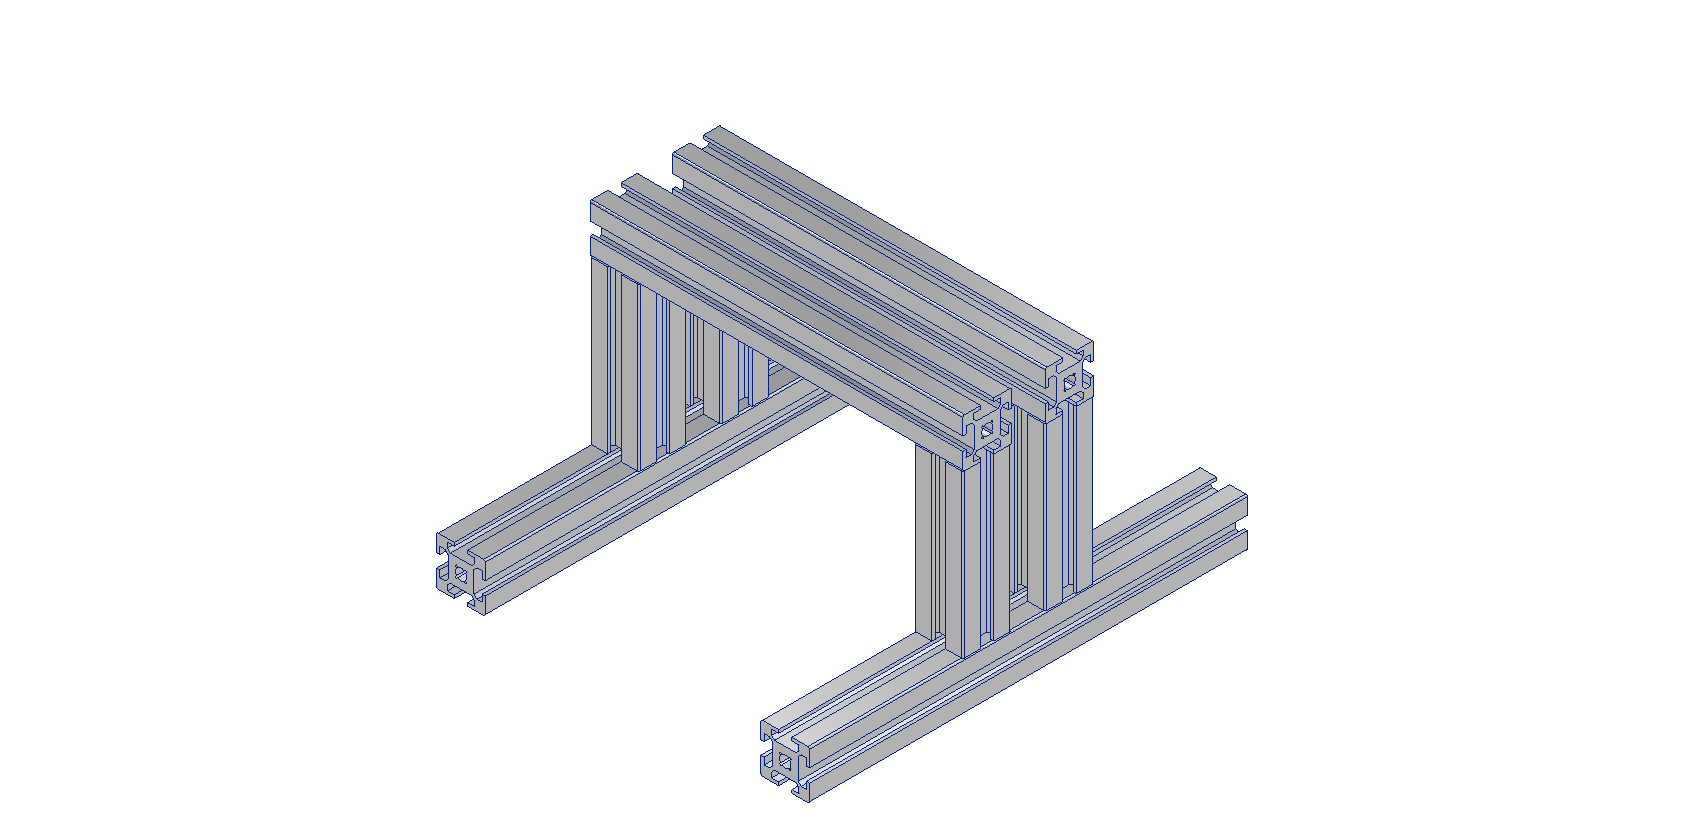
\includegraphics[
				width=\linewidth,
				height=65mm,
				keepaspectratio
			]{Resultados/Integración/BaseBaja.png}
			\caption{Base para el Módulo inferior}
			\label{fig:DiagramaRayos}
		\end{figure}
		
		Finalmente en la~\cref{fig:VistaCompleta} se observa la integración completa al seguidor solar.
		
		\begin{figure}[H]
			\centering
			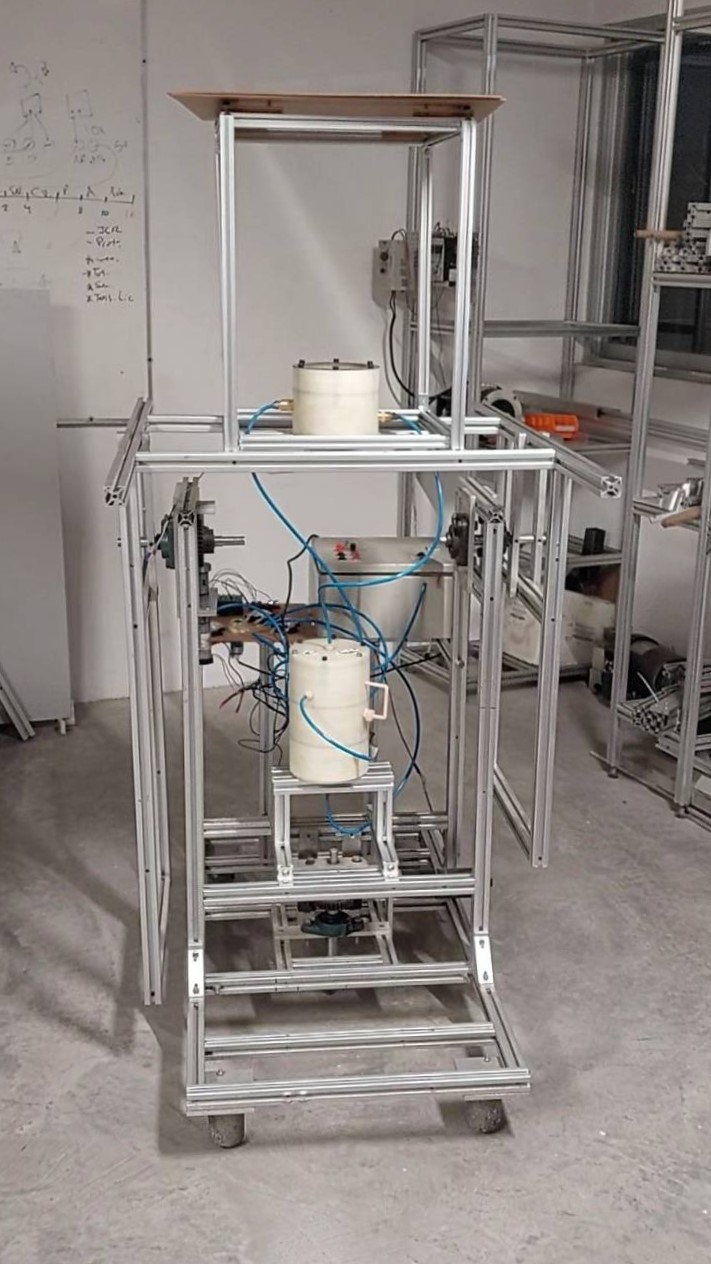
\includegraphics[
				width=\linewidth,
				height=65mm,
				keepaspectratio
			]{Resultados/Integración/VistaCompleta.jpg}
			\caption{Vista lateral del ensamble completo}
			\label{fig:VistaCompleta}
		\end{figure}

			
%			\begin{figure}[H]
%				\centering
%				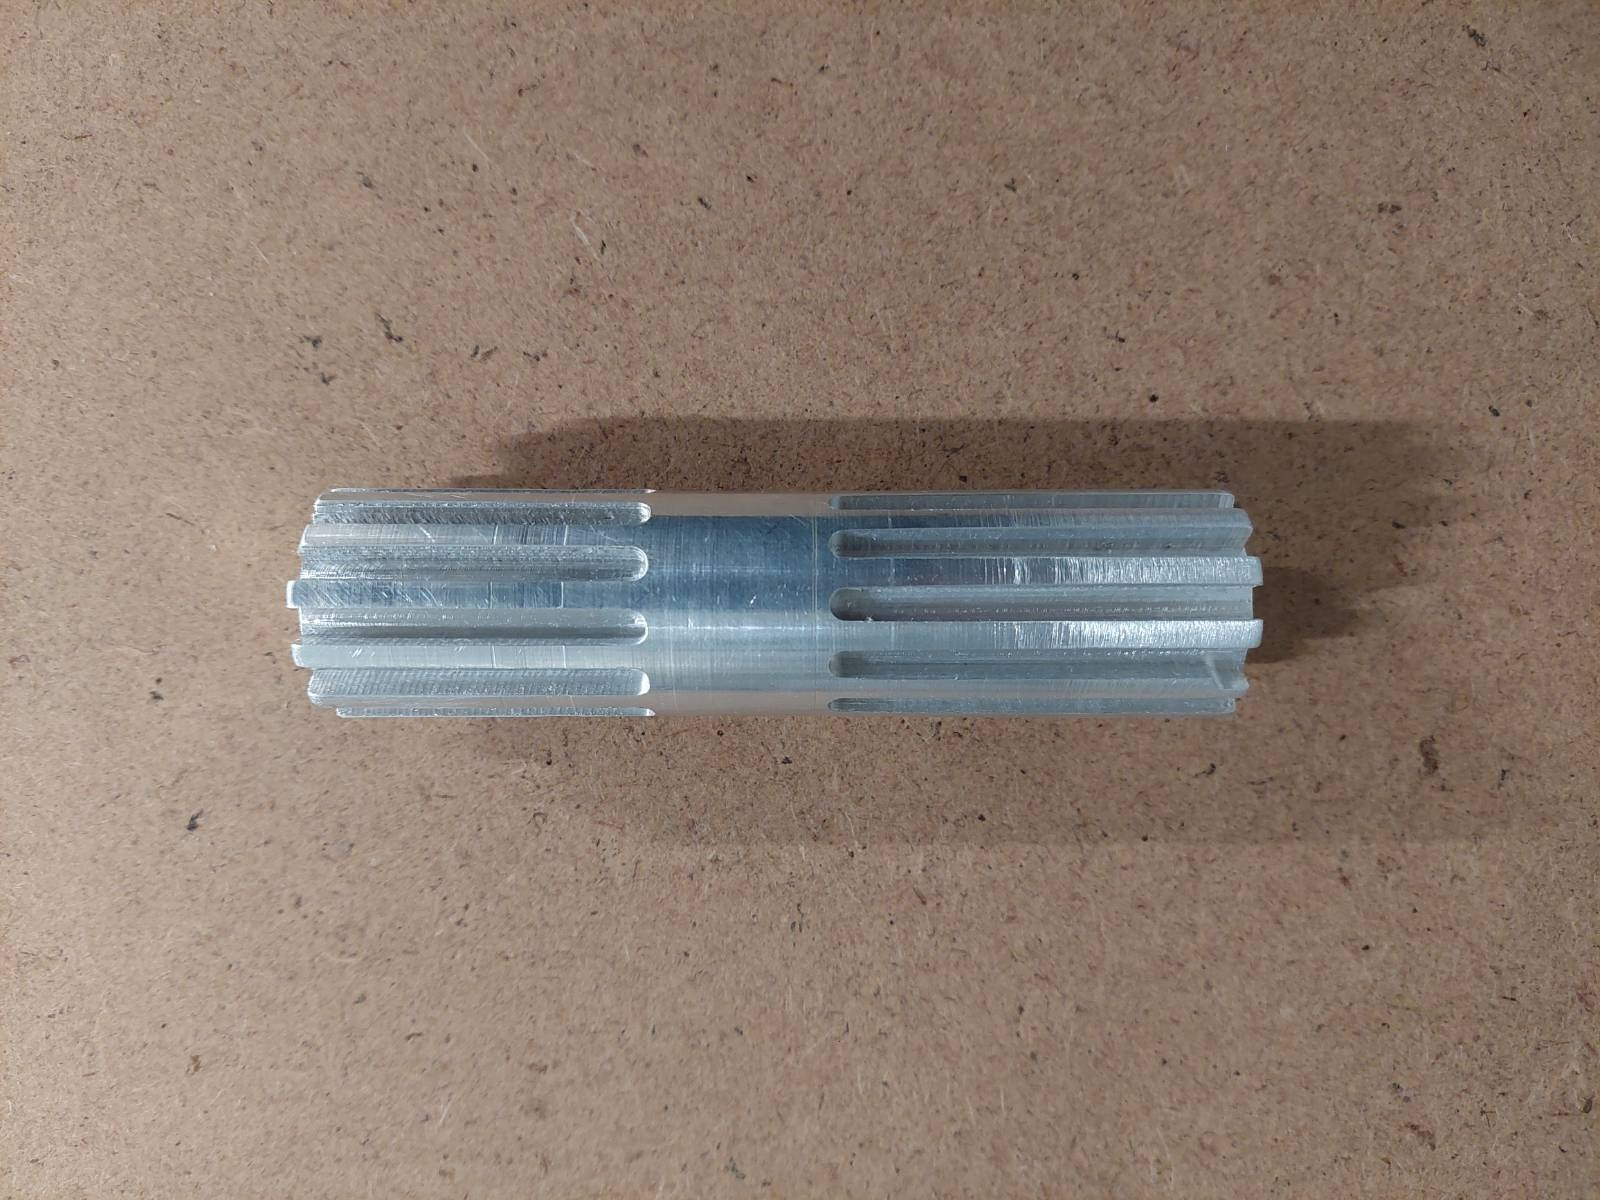
\includegraphics[
%					width=\linewidth,
%					height=65mm,
%					keepaspectratio
%				]{Resultados/Construcción/Intercambiador-de-calor.jpg}
%				\caption{Intercambiador de calor con aletas verticales}
%				\label{fig:Intercambiador-de-calor.jpeg}
%			\end{figure}
			
			